%!TEX root = ../main.tex

\chapter{A brief introduction to superconducting qubits} % (fold)
\label{cha:SCQubitPrinciple}
  
% chapter SCQubitPrinciple (end)

This appendix is designed to be a concise introduction to superconducting qubits with a focus on transmon qubits, including the theoretic derivation of its Hamiltonian and properties, a brief history of the development of transmon qubits and crucial technical improvements. See, for example, Ref.~\inlinecite{Clarke2008,devoret2013superconducting,Wendin2016} for a more detailed review about superconducting qubits.

This appendix is written as a `router' for more detailed literature on topics included, with the most important results and conclusions explicitly presented here.

\section{Principle of superconducting qubits} % (fold)
\label{sec:principle_of_superconducting_qubit}
    
    When talking about a qubit, and more generally quantum information processing, the first thing is the criteria for a good qubit, which is originally proposed by DiVincenzo\cite{divincenzo2000physical} and is known as the DiVincenzo criteria
    \begin{enumerate}
        \item Qubits: fabrication of registers with several (many) qubits
        \item Initialization: the qubit register must be possible to initialise to a known state
        \item Universal gate operations: high fidelity single and 2-qubit gate operations available
        \item Readout: the state of the qubit register must be possible to read out, typically via readout of individual qubits
        \item Long decoherence times: large number of single and 2-qubit gate can be performed within the qubit decoherence time
        \item Quantum interfaces for qubit interconversion
        \item Quantum interfaces to flying qubits for optical communication
    \end{enumerate}
    I'll try to cover the above seven points for superconducting qubits.


    \subsection{Hamiltonian of Transmon} % (fold)
    \label{sub:hamiltonian_of_transmon}
    A superconducting qubits can be viewed as a superconducting nonlinear oscillator. For a simple linear oscillator, the Hamiltonian is
    \begin{equation}
    \label{eqn:linearOscillatorHam}
        H = 4E_C \hat n^2 + E_L \frac{\hat \delta^2}{2}
    \end{equation}
    where $\hat n$ is the excess charge on the capacitor in units of 2e and $ \hat \delta  $ is the phase difference of the inductor. $E_C = e^2/2C$ is the charging energy\cite{koch2007charge} and $E_L = \Phi_0^2/4 \pi^2 L $ is the energy of one flux quantum. You might see $\hat n - n_g$ instead of $\hat n$ in literature, where $\hat n$ is total charge operator and $n_g$ is the effective offset charge controlled by a capacitively coupled gate. Also in some literature, charging energy $E_C$ is defined as $ (2e)^2/2C $ so that there's no factor $4$ before the charge term of the Hamiltonian (see, e.g., Ref.~\inlinecite{Wendin2016,Collin2004}).

    This harmonic oscillator Hamiltonian leads to evenly spaced energy levels and can not be used as a qubit with effectively two levels. A nonlinear element called Josephson junction (J-J) is utilized to bring aharmonicity to the system. A J-J is realized by separating two superconducting regions with a thin insulator. The insulator is thin enough to allow the tunneling of Cooper pairs across the junction. The most important phenomena in a J-J is the current-phase and voltage-phase relation (see Appendix A of Ref.~\inlinecite{Raab2015} for a brief derivation):
    \begin{align}
    \label{eqn:currentVoltagePhase}
        I &= I_c \sin \delta \\
        \dot \delta & = \frac{2e}{\hbar} V = \frac{2 \pi}{\Phi_0} V
    \end{align}
    Where $ \delta $ is the phase difference across the junction. As a result, the energy of a J-J is\cite{Raab2015}
    \begin{equation}
        H_J = \int dt VI = \frac{\Phi_0 I_c}{2 \pi}\int dt \dot \delta \sin \delta = -\frac{\Phi_0 I_c}{2 \pi}\cos \delta = -E_J \cos \delta
    \end{equation}
    Hence when using a J-J as an nonlinear inductance, the Hamiltonian (\ref{eqn:linearOscillatorHam}) becomes
    \begin{equation}
        H = 4E_C \hat n^2 -E_J \cos \hat \delta  
    \end{equation}

    The exact solution of the energy levels of the above Hamiltonian includes Mathieu functions\cite{schuster2007circuit,koch2007charge}. For transmon qubits with $E_J /E_C \sim 100$, the energy levels simplified to\cite{koch2007charge}
    \begin{equation}
    \label{eqn:transmonLevels}
        E_m \approx -E_J + \sqrt{8E_CE_J} \left (m+\frac{1}{2} \right ) - \frac{E_C}{12}(6m^2+6m+3)
    \end{equation}
    where $ \omega_p = \sqrt{8E_CE_J}/\hbar   $ is known as the plasma frequency. Absolute and relative anharmonicity is often defined to characterize the transmon anharmonicity, which are
    \begin{align}
        \alpha &\equiv E_{12} - E_{01} \approx -E_C\\
        \alpha_r & \equiv \alpha/E_{01} \approx -(8E_J/E_C)^{-1/2}
    \end{align}
    
    In some superconducting qubit design, two J-J are used to form a SQUID. The Hamiltonian of a SQUID is\cite{koch2007charge}
    \begin{equation}
        H_J = -E_{J1}\cos \delta_1 -E_{J2}\cos \delta_2
    \end{equation}
    where $ \delta_{1,2} $ now describe the phase difference across the junctions. Flux quantization then require (see Appendix A of Ref.~\inlinecite{Raab2015} for a simple derivation)
    \begin{equation}
        \delta_1 - \delta_2 = 2 \pi n + 2 \pi \Phi/\Phi_0
    \end{equation}
    where $n$ is an integer, $\Phi $ is the flux through the SQUID ring which is adjustible by, e.g.,  a nearby wire, and $ \Phi_0 =h/2e  $ is the superconducting flux quantum. Define the effective phase difference $ \delta = (\delta_1+\delta_2)/2 $, $E_{J \Sigma} = E_{J1} + E_{J2} $ and the junction asymmetry $d = (E_{J2}- E_{J1})/(E_{J2}+E_{J1}) $ which is typically 10\%, the SQUID Hamiltonian can be written as\cite{koch2007charge}
    \begin{equation}
        H_J = - E_{J \Sigma} \cos \left (\frac{\pi \Phi}{\Phi_0} \right )\sqrt{ 1+d^2 \tan^2 \left (\frac{\pi \Phi}{\Phi_0} \right ) }\cos(\hat \delta - \delta_0)
    \end{equation}
    where $ \delta_0 $ determined by $ \tan \delta_0 = d \tan(\pi \Phi/\Phi_0) $. The presence of $ \delta_0 $ in SQUID with asymmetric junctions can lead to additional qubit control and hence additional decay channel. As a result, using a symmetric SQUID instead of a simple J-J gives rise to qubits with tunable junction energy $ E_J = E_{J \Sigma} \cos(\pi \Phi/\Phi_0) $.

        
    % subsection hamiltonian_of_transmon_and_transmon_in_cqed (end)
    

    \subsection{Control and readout of transmon qubits} % (fold)
    \label{sub:control_and_readout_of_transmon_qubits}

        A schematic figure of transmon circuit is shown in Fig.~\ref{fig:transmonSchematic}.

            \begin{figure}[h]
                \centering
                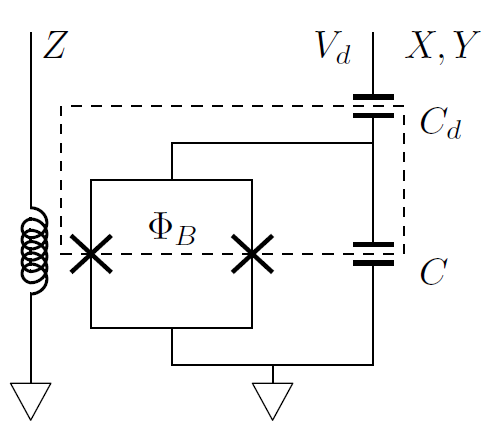
\includegraphics[width=3in]{transmon_scheme.png}
                \caption{Transmon circuit with X, Y and Z control, adapted from Ref.~\inlinecite{Raab2015}.}
                \label{fig:transmonSchematic}
            \end{figure}
            Where the drive voltage $V_d$ can come from both a microwave cavity field\cite{koch2007charge} and an independent drive line\cite{Barends2013Coherent}. The X control is realized by flux-biasing the SQUID, temporarily changing the transmon energy spacing according to eqn.~(\ref{eqn:transmonLevels}). Following Ref.~\inlinecite{Raab2015}, the Hamiltonian of the transmon with drive $ V_d $ is
            \begin{equation}
            \label{eqn:transmonWithDrive}
                H = 4E_C \hat n^2  - E_J \cos \delta + \frac{C_d}{C_\Sigma} 2eV_d \hat n
            \end{equation}
            where the charge operator $\hat Q$ in Ref.~\inlinecite{Raab2015} is substituted to $ 2e \hat n $. Eqn.~(\ref{eqn:transmonWithDrive}) is comparable to Eqn.~(3.1) in Ref.~\inlinecite{koch2007charge}, which I also include here:
            \begin{equation}
            \label{eqn:transmonWithCavityDrive}
                H = 4E_C (\hat n - n_g)^2 - E_J \cos \delta +2 \beta e V^0_{\text{rms}}\hat n( \hat a + \hat a^\dagger ) + \hbar \omega \hat a^\dagger \hat a
            \end{equation}
            where $n_g$ is the charge offset neglected in eqn.~(\ref{eqn:transmonWithDrive}). $ \beta = C_d/C_\Sigma $ is the ratio between the gate capacitance and the total capacitance. $V^0_{\text{rms}} $ is the zero-field root-mean-square voltage, hence $V^0_{\text{rms}}( \hat a + \hat a^\dagger ) = V_d$. The extra term $H_r = \hbar \omega \hat a^\dagger \hat a$ comes from the microwave resonator the transmon coupled to, which in not taken into account in Fig.~\ref{fig:transmonSchematic}.

            Expanding the Hamiltonian in transmon basis $ \ket{i} $, the Hamiltonian becomes
            \begin{align}
            \label{eqn:transmonWithCavityDriveExpanded}
                H &= \hbar \sum_j \omega_j \ket j \bra j + \hbar \omega_r \hat a^\dagger \hat a + \hbar \sum_{i,j} g_{ij} \ket i \bra j (\hat a + \hat a^\dagger ) \\
                \label{eqn:simplifiedTransmonWithCavityDrive}
                & \approx \hbar \sum_j \omega_j \ket j \bra j + \hbar \omega_r \hat a^\dagger \hat a  + \left (\hbar \sum_{i} g_{i,i+1} \ket i \bra{i+1} \hat a^\dagger + h.c. \right )
            \end{align}
            where $\hbar g_{ij} = 2 \beta e V^0_{\text{rms}} \bra i \hat n \ket j$. The approximation $ |\bra{j+k}\hat n \ket j| \rightarrow 0  $ when $|k|>1, E_J/E_C \rightarrow \infty $ and rotating wave approximation (RWA) are adopted. The non-vanishing coupling matrix elements are
            \begin{equation}
            \label{eqn:couplingElements}
                | \bra{j+1} \hat n \ket j |\approx \sqrt{ \frac{j+1}{2}} \left ( \frac{E_J}{8E_C} \right )^{1/4} 
            \end{equation}

            When the state space is further restricted to the ground and first excite state, the Hamiltonian (\ref{eqn:simplifiedTransmonWithCavityDrive}) reduce to the Jaynes-Cummings Hamiltonian\cite{walls2007quantum,schuster2007circuit}
            \begin{equation}
            \label{eqn:JCHamiltonian}
                H = \hbar \frac{\omega_{01}}{2} \hat \sigma_z + \hbar \omega_r \hat a^\dagger \hat a  + \hbar (g_{01}\hat a^\dagger \hat \sigma^- + h.c. )
            \end{equation}
            where $ \hbar \omega_{01} = \sqrt{8E_JE_C} - E_C $ is the qubit energy separation.
            
            If we start from eqn.~(\ref{eqn:simplifiedTransmonWithCavityDrive}) but without the RWA, switch back to classical drive field $V_d = V_{d0}\cos(\omega_d t + \phi) $ without the cavity and keep only the lowest two levels, the Hamiltonian turns to
            \begin{align}
                H &= \hbar \frac{\omega_{01}}{2} \hat \sigma_z + 2 \beta e \sqrt{ \frac{1}{2}} \left ( \frac{E_J}{8E_C} \right )^{1/4} V_{d0} \hat \sigma_x \cos(\omega_d t + \phi) \\
                &=   \hbar \frac{\omega_{01}}{2} \hat \sigma_z + \Omega \hat \sigma_x \cos(\omega_d t + \phi)
            \end{align}
            Transforming into the rotating frame with the drive frequency by applying $ U = \exp(i \omega_d t \hat \sigma_z /2) $ such that $ H_{RF} = UHU^\dagger + i\hbar \dot U U^\dagger $, the Hamiltonian becomes
            \begin{align}
                H_{RF} &= \hbar \frac{\omega_{01} - \omega_d}{2} \hat \sigma_z + \Omega ( \cos (\omega_d t) \hat \sigma_x - \sin (\omega_d t) \hat \sigma_y )\cos(\omega_d t + \phi)\\
                & = \hbar \frac{\omega_{01} - \omega_d}{2} \hat \sigma_z + \frac{\Omega}{2} \cos \phi \hat \sigma_x+ \frac{\Omega}{2} \sin \phi \hat \sigma_y
            \end{align}
            where the terms rotating at $ 2 \omega_d t $ is thrown away by RWA. The resulting Hamiltonian shows that the drive effectively rotate the qubit state along the axis $B_{\text{eff}} = ((\omega_{01} - \omega_d)/2,\Omega \cos \phi /2,\Omega \sin \phi /2)$, like a spin-1/2 particle in the effective magnetic field $B_{\text{eff}}$, realizing the X and Y drive.

            In most circumstances, a transmon qubit is coupled to a microwave resonator for readout, and the corresponded Hamiltonian is identical to eqn.~(\ref{eqn:JCHamiltonian}). When the resonator and transmon are detuned from each other, the J-C Hamoltonian goes to the dispersive limit\cite{Blais2004,schuster2007circuit}
            \begin{equation}
                H \approx \hbar \left (\omega_r + \frac{g_{01}^2}{\Delta} \hat \sigma_z \right )\hat a^\dagger \hat a+ \frac{1}{2} \hbar \left(\omega_{01} + \frac{g_{01}^2}{\Delta}\right) \hat \sigma_z
            \end{equation}
            where $ \Delta = \omega_{01} - \omega_r \gg g_{01}$ is the transmon-cavity detuning. Explicitly, the cavity resonant frequency depends on the state of the transmon, hence by probing the cavity response, the state of the transmon can be extracted. Single-shot readout can be achieved by proper amplification process\cite{Mallet2009,Sliwa2016}.


        
    % subsection control_and_readout_of_transmon_qubits (end)

    \subsection{Decay and dephasing in transmon qubits} % (fold)
    \label{sub:decay_and_dephasing_in_transmon_qubits}

    Decay and dephasing are both large topics and won't be covered here for detail.

    Chapter 4 in Ref.~\inlinecite{schuster2007circuit} theoretically discussed decoherence in superconducting qubits in great detail, including voltage noises, material loss, dipole radiation, charge and flux noise and $E_J$ and $E_C$ noise. Transmon was proposed to fight against charge noise.

    Ref.~\inlinecite{Martinis2014Report} discussed decoherence in transmon qubit experimentally. Capacitor loss, inductor and junction loss, and radiation and wiring loss were discussed. Many technical details are involved to obtain qubits with higher coherence and these details will be mentioned in \ref{sec:technical_improvements}.
    
    % subsection decay_and_dephasing_in_transmon_qubits (end)
    

% section principle_of_superconducting_qubit (end)


\section{A brief history of the development of transmon qubits} % (fold)
\label{sec:history_of_the_development_of_transmon_qubit}

The superconducting qubits evolves from Cooper pair box (CPB), which is basically a charge island separated from a charge reservoir by a J-J. Early research about CBP (originally called superconducting single-electron box\cite{Nakamura1997}) mainly concerned about its transport properties and charging effects. In 1999, pulse modulation of quantum states were realized by Nakamura \etal\cite{Nakamura1999}. A gate voltage pulse brought two levels of the CPB into resonance and coherent oscillations in state population was observed by varying the pulse length. The coherence time was $\sim 1$ns. To obtain better coherence, the same group used spin-echo-type technique on the same system and identified the dominant dephasing source was the $1/f$ charge noise\cite{Nakamura2002}. More works quickly followed on similar system, with microwave pulses manipulating the qubit state\cite{Vion2002,Collin2004} and also with more complex device such as two coupled charge qubit\cite{Pashkin2003}. Ref.~\inlinecite{Makhlin2001} is a review about early but also fundamental superconducting qubit design.


            \begin{figure}[h]
                \centering
                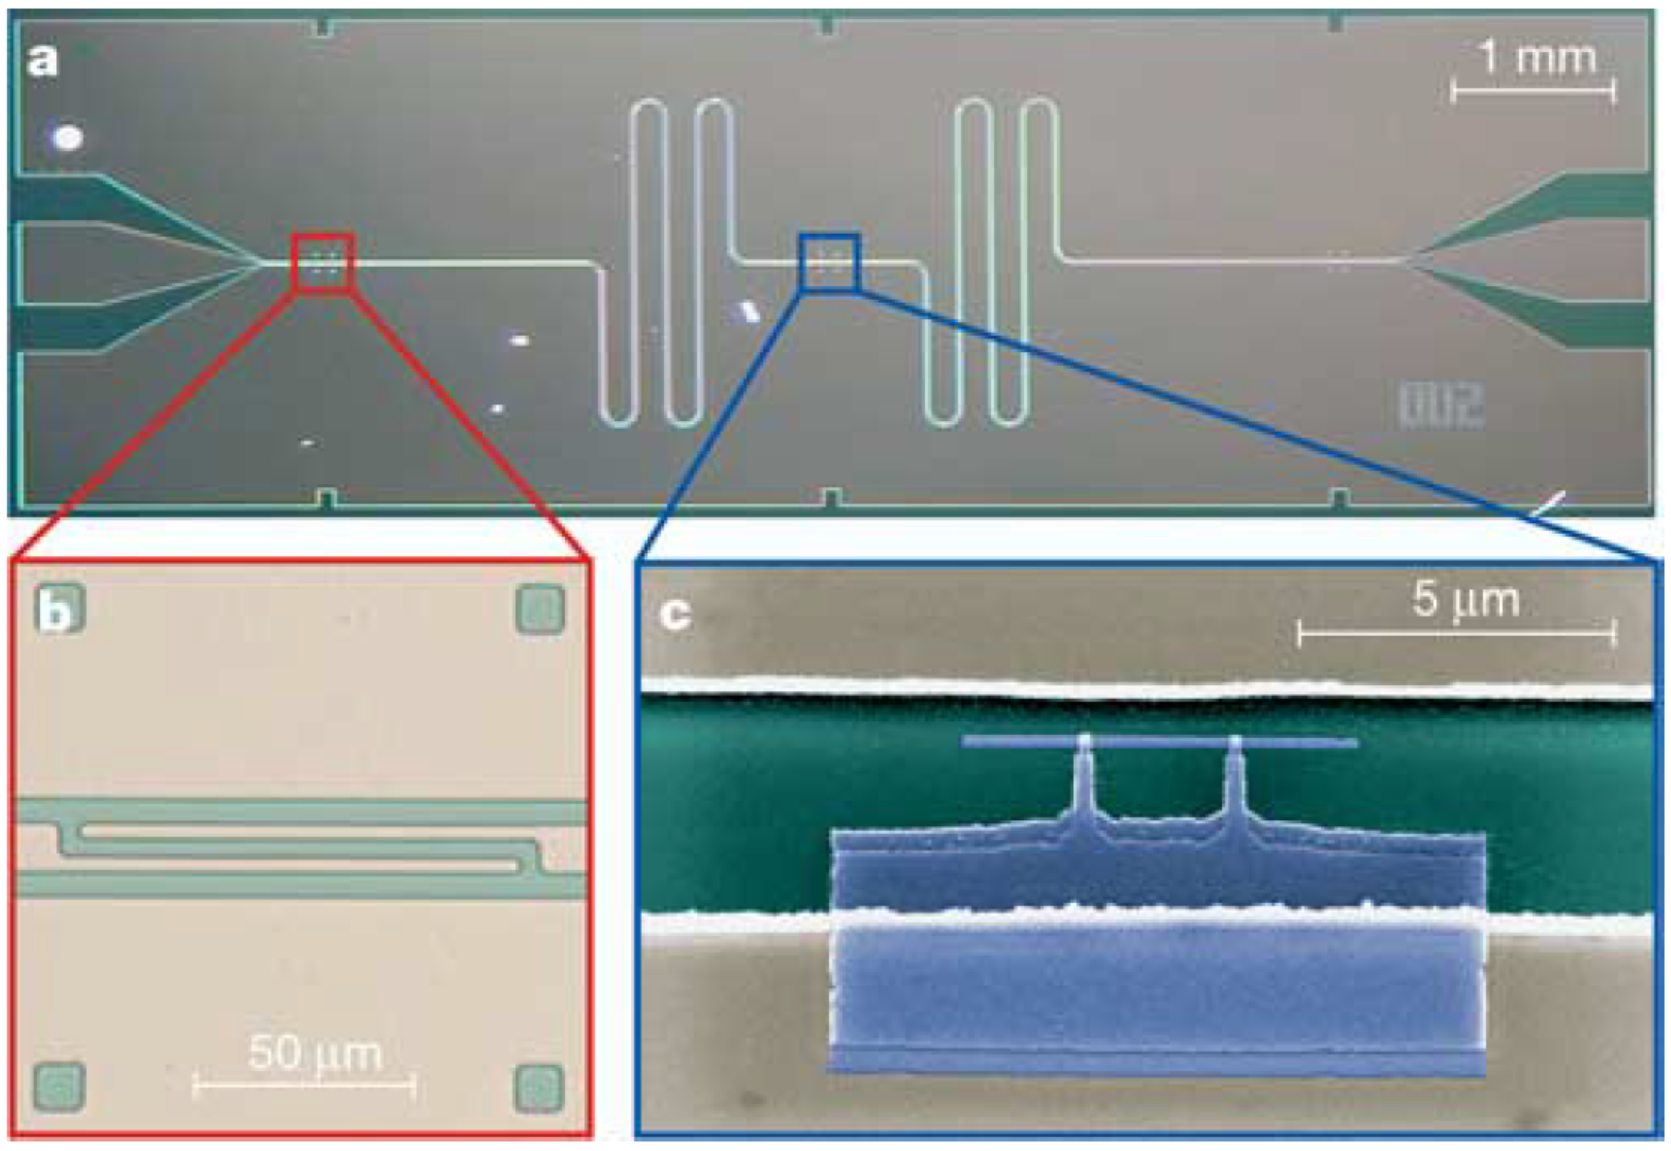
\includegraphics[width=4in]{review/strongCoupling2004.png}
                \caption{Strong coupling between superconducting qubit and single photon, adapted from Ref.~\inlinecite{Wallraff2004Nature}.}
                \label{fig:strongCoupling2004}
            \end{figure}

In 2004, Yale group proposed circuit quantum electrodynamics (cQED) as an architecture for quantum computation, where superconducting qubits are coupled to CPW resonator for control and readout\cite{Blais2004}. In the same year, strong coupling between superconducting charge qubit and CPW resonator was achieved\cite{Wallraff2004Nature}. By probing the cavity transmission while manipulating the qubit level structure via gate voltage and flux bias, level structure and vacuum Rabi splitting were clearly observed. In their following experiments, effect of the ac Stark shift from the cavity on the qubit and hence the dephase from the photon shot noise is experimentally explored\cite{Schuster2005} and theoretically explained\cite{Gambetta2006}. The qubit line shape fits better to a Lorentzian (Gaussian) for low (high) intra-cavity photon number, which agrees with their theory of measurement-induced dephasing. The dephasing time exceeded 200ns in this work.


In 2007, The same group at Yale proposed more detailed single and two qubit(s) gate design for quantum information processing based on cQED\cite{Blais2007}. At the same time, coupling between remote qubits were realized with both phase qubits\cite{Sillanpaa2007} and charge qubits\cite{Majer2007} via a cavity bus. While probing the cavity resonance can be used for qubit readout, Schuster \etal{} showed that the qubit spectroscopy can be used to resolve photon number states of the cavity\cite{Schuster2007Resolving}.


            \begin{figure}[h]
                \centering
                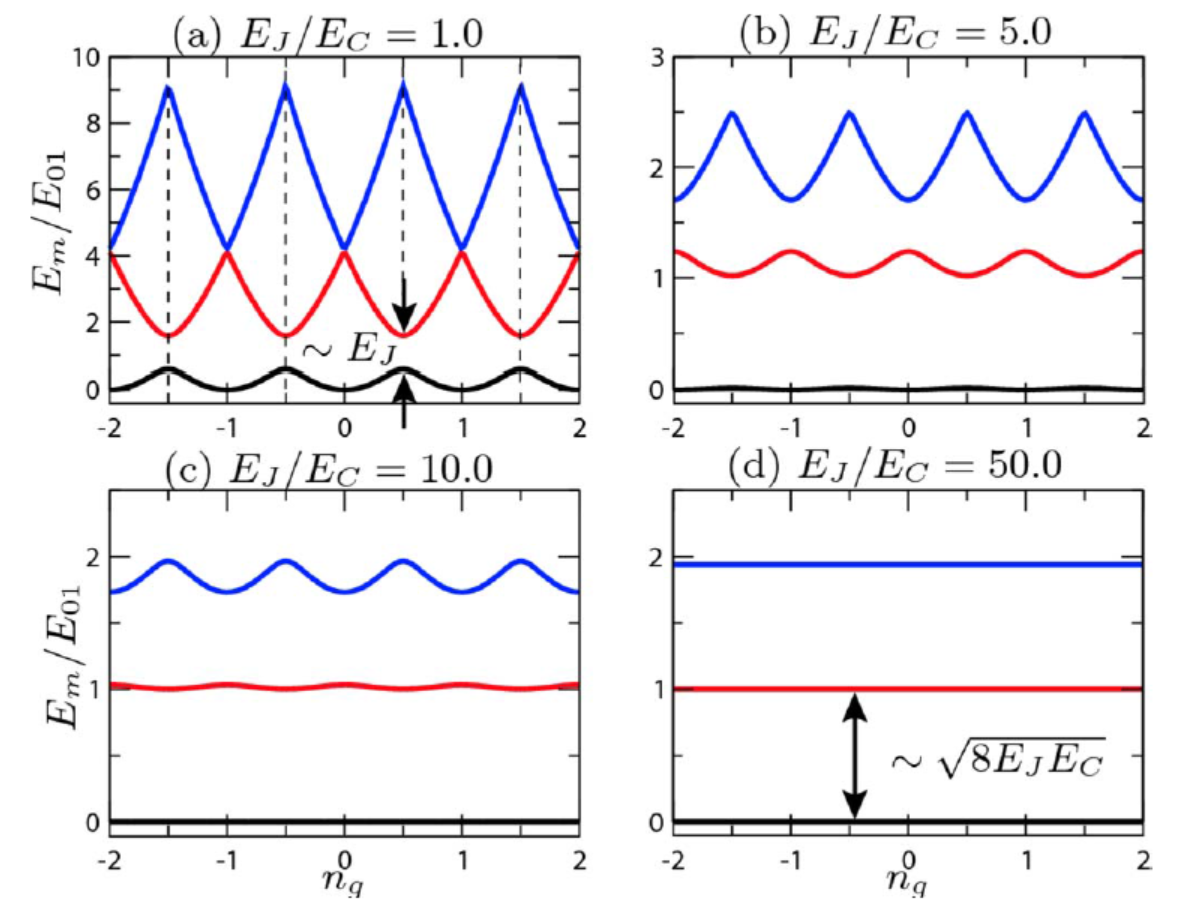
\includegraphics[width=4in]{review/transmon2007.png}
                \caption{Energy levels of superconducting qubit versus gate charge, with different $E_J/E_C$ value. Adapted from Ref.~\inlinecite{koch2007charge}.}
                \label{fig:transmon2007}
            \end{figure}


The charge qubits suffer from $1/f$ charge noise, since the energy levels depends on the gate induced charge $n_g$. Degrees of control always correspond to channels of dephasing. In order to suppress the sensitivity to charge noise, Koch \etal{} proposed transmon qubits\cite{koch2007charge}. The ratio between $E_J$ and $E_C$ is increased to suppress the dependence of energy levels with respect to $n_g$, while the anharmonicity still remains sufficient for defining qubits. Their proposal was quickly implemented approximately one year later\cite{Schreier2008}, where the various decay and dephasing times are all above 1$\mu$s.


            \begin{figure}[h]
                \centering
                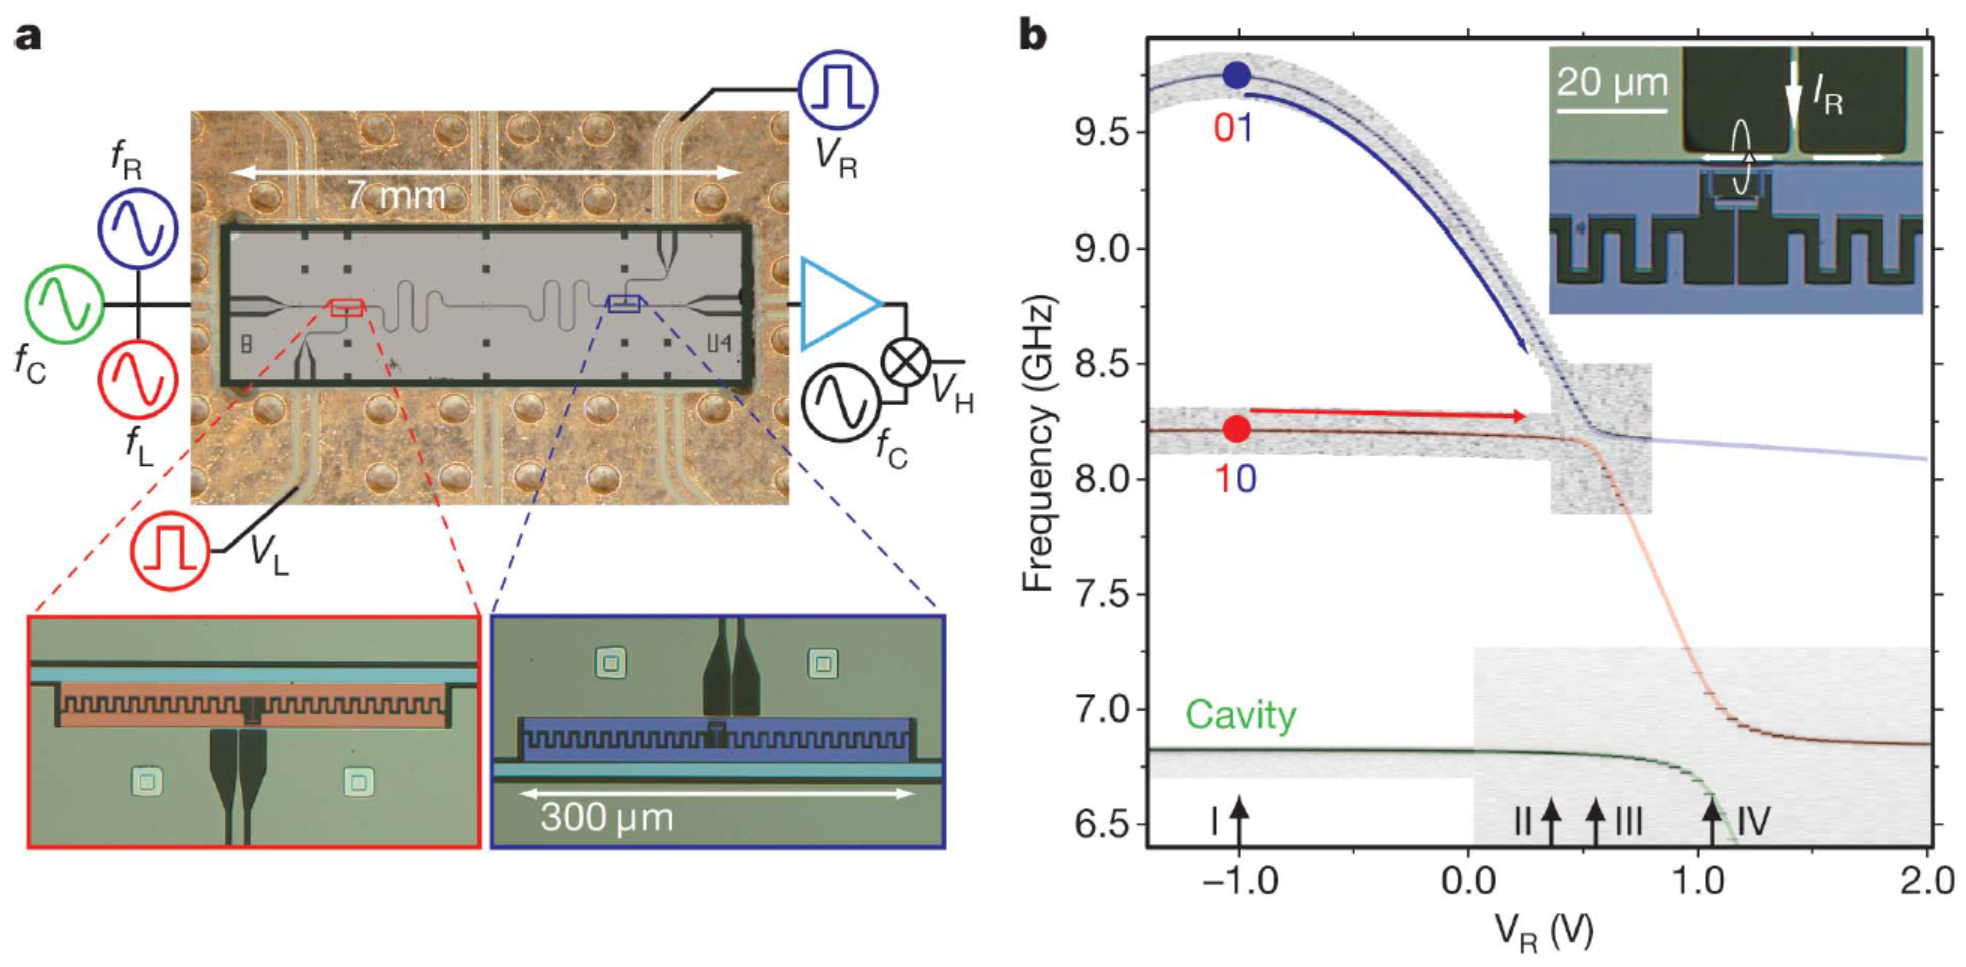
\includegraphics[width=5in]{review/twoQubit2009.png}
                \caption{Device for demonstration of two-qubit algorithms. Adapted from Ref.~\inlinecite{DiCarlo2009}.}
                \label{fig:twoQubit2009}
            \end{figure}

With the new transmon design and multiple qubit coupling, the Yale group soon proceeded to multi-qubit manipulations and readout. Two-qubit state tomography using a joint disppersive readout was proposed in Ref.~\inlinecite{Filipp2009}, where the cavity frequency shift depends on both states of the two qubits coupling to the cavity. With two transmons coupled to a cavity bus, DiCarlo \etal{} showed two-qubit algorithm in superconducting system\cite{DiCarlo2009}. Two qubit controlled phase gate was implemented utilizing level pulling from a non-computational state by adiabatic flux pulse. They soon went to couple four transmons in one cavity and succesfully prepared and measured a three-qubit entanglement\cite{DiCarlo2010}. The flux-pulse C-Phase gate was 12ns in their case and the qubit coherence time is on the level of $\sim 1 \mu$s.


            \begin{figure}[h]
                \centering
                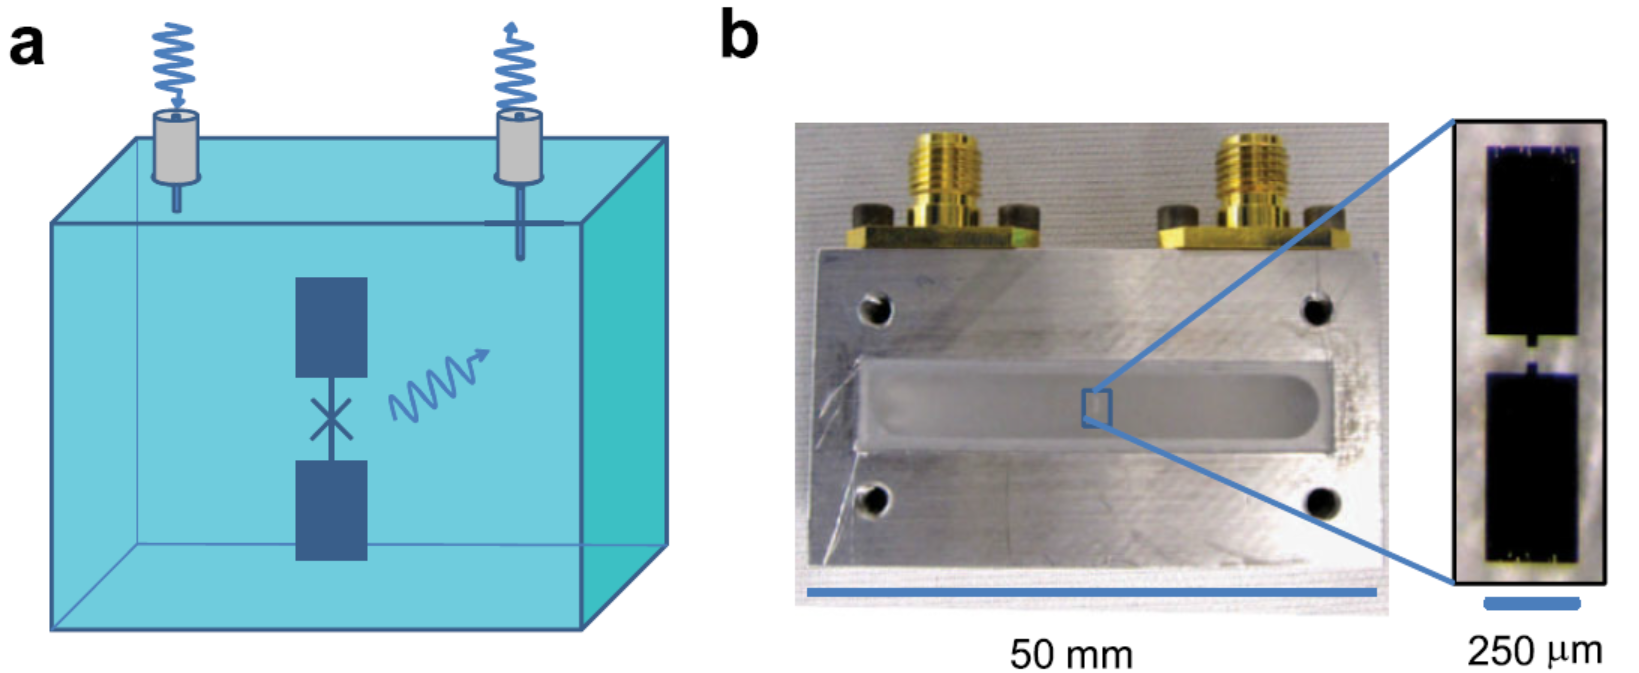
\includegraphics[width=4in]{review/3D_transmon2011.png}
                \caption{3D transmon design. Adapted from Ref.~\inlinecite{DiCarlo2009}.}
                \label{fig:Paik2011}
            \end{figure}

While the coherence time of superconducting qubits has been steadily improved from $\sim 1$ns in original CPB to $\sim 1 \mu$s for transmons, the Yale group made another drastic improvement by the 3D transmon design\cite{Paik2011}. The measured $T_1$ was up to $60\mu$s and $T_2 \sim 10\mu$s. The long coherence time benefitted from the avoidance of $1/f$ charge noise, single junction design and also material optimizations. The record and was soon further increased to $\sim 0.1$ms\cite{Rigetti2012} by reducing dephasing rate per residual cavity photon, minimize coupling to higher cavity mode and lowering the thermal photon temperature of the cavity.



            \begin{figure}[h]
                \centering
                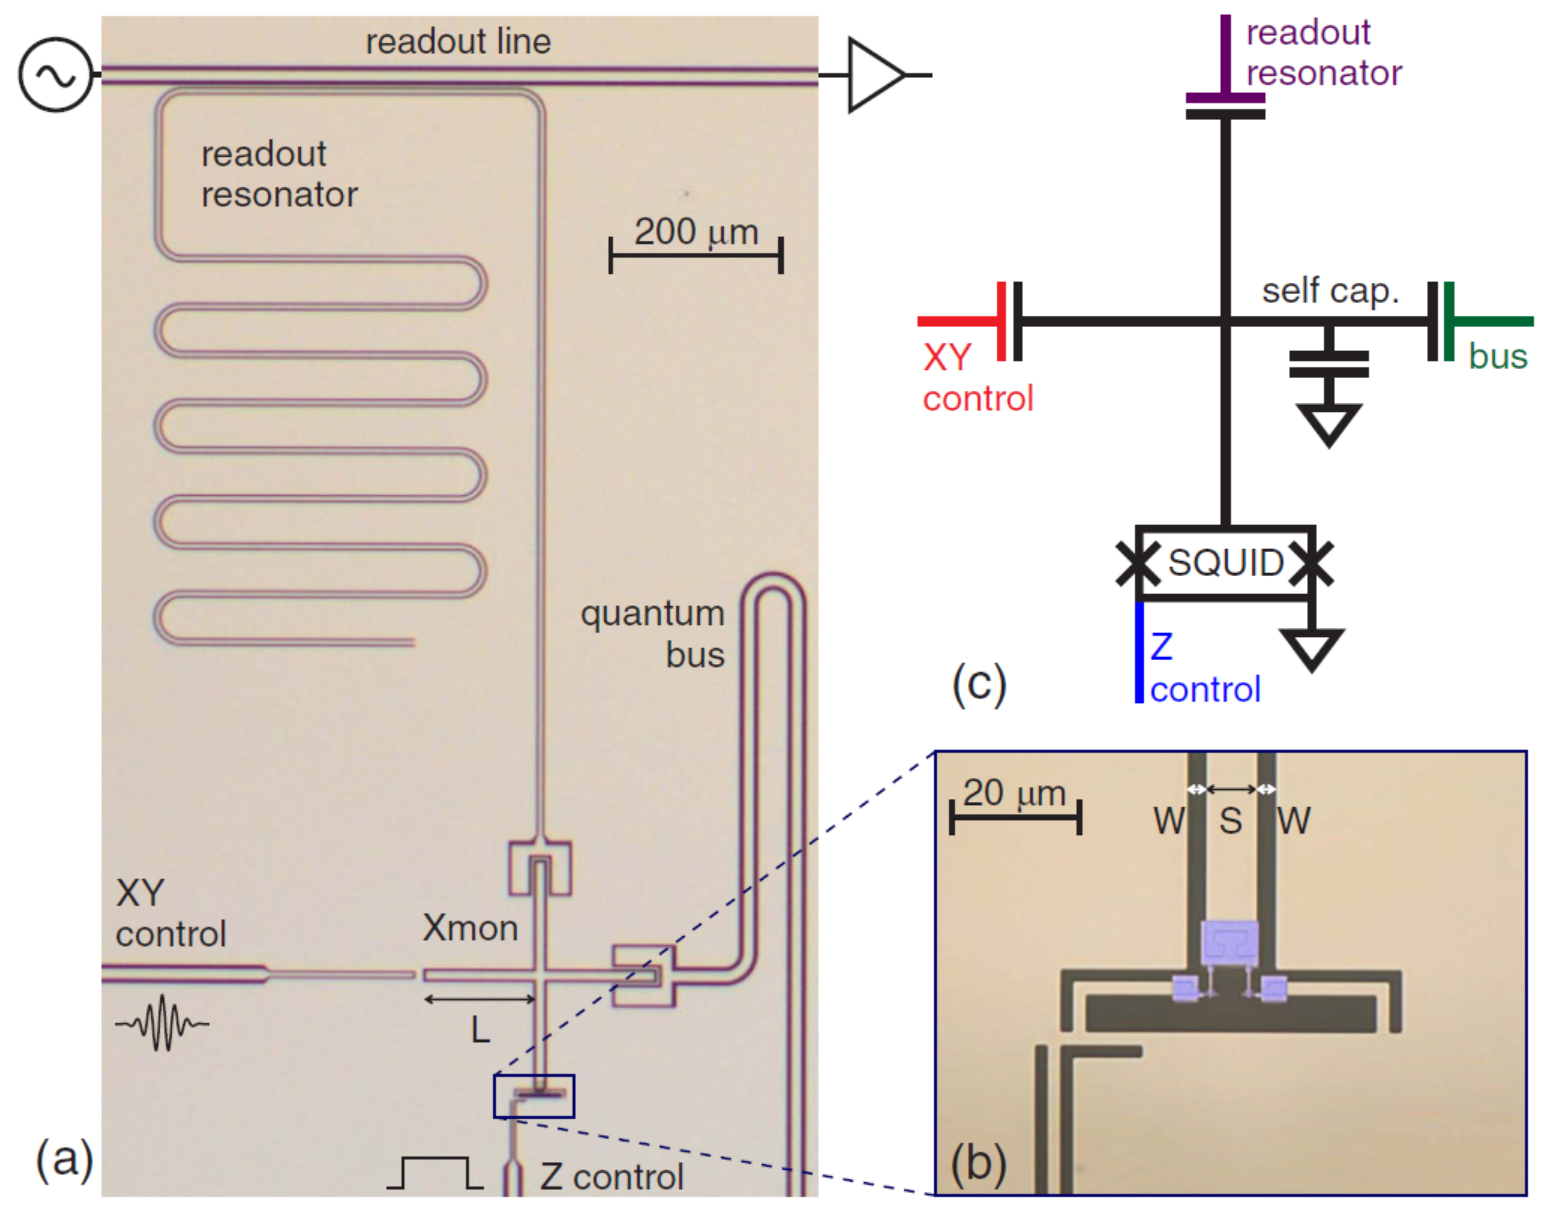
\includegraphics[width=4in]{review/XmonDesign2013.png}
                \caption{Xmon design. Adapted from Ref.~\inlinecite{Barends2013Coherent}.}
                \label{fig:XmonDesign2013}
            \end{figure}




Besides the Yale group, there are also many other groups working on superconducting qubits, in which Prof. Martinis' group at UCSB stands out. Beyond their previous interests in phase qubits, the UCSB group proposed a variation of transmon named Xmon\cite{Barends2013Coherent}, which was designed for scalability with surface code\cite{Fowler2012}. In the Xmon design, the resonator for qubit readout is modified from in-line reflection type to hanger type, allowing one transmission line to couple with many hanger resonators. The `X' shape of the qubit capacitor offers coupling to readout resonator, quantum bus, XY drive and Z control respectively. With a lot of technical improvements (see Sec.~\ref{sec:technical_improvements}), the Xmon qubit showed coherence time $\sim 15\mu$s. Based on the Xmon design, the same group at UCSB increased the number of coupled Xmon qubits to five\cite{Barends2014} and nine\cite{Kelly2015} in 2014 and 2015 respectively. These qubits have coherence time $\sim 30\mu$s, single qubit gates fidelity all above 0.999 and two-qubit gate fidelity above 0.99 between all coupled qubits.


            \begin{figure}[h]
                \centering
                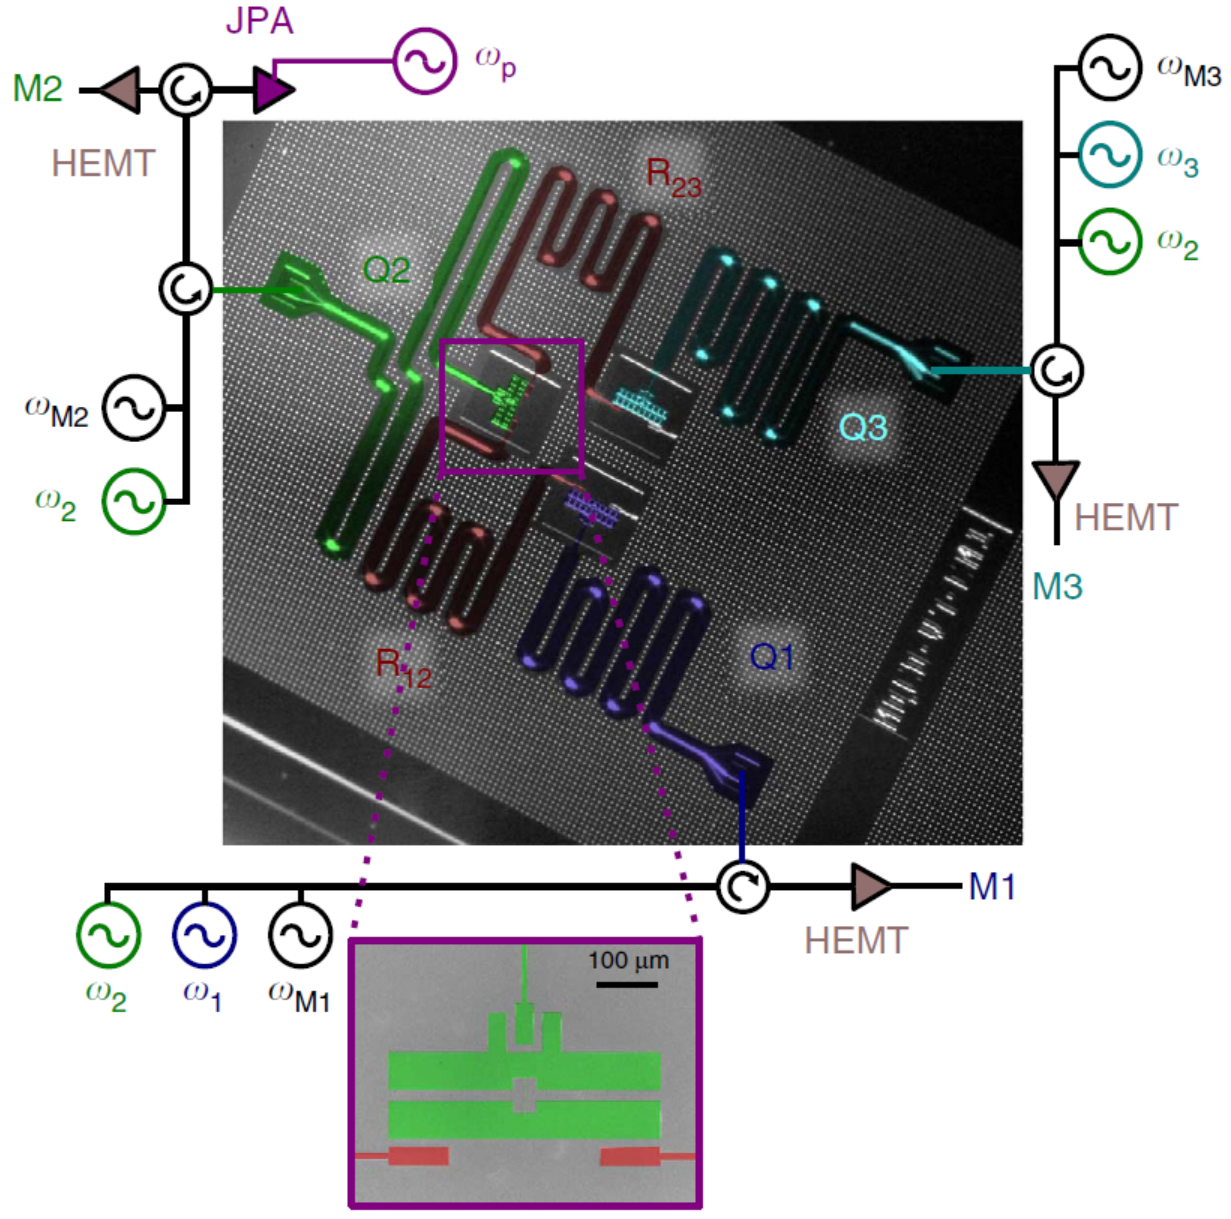
\includegraphics[width=4in]{review/IBMTransmon2014.png}
                \caption{The IBM transmon design. Adapted from Ref.~\inlinecite{Chow2014}.}
                \label{fig:IBMTransmon2014}
            \end{figure}


Another group at IBM adopted the 3D transmon design on 2D\cite{Chow2014,Takita2017} and was followed by other groups\cite{Mlynek2014,Pechal2016,Walter2017}. Based on their design, IBM initiated IBM Q in 2015 and provided a 5-qubit processor to public access\cite{IBMQ}. Recently they announced that they've successfully built and tested a 16-qubit processor for developers, researchers, and programmers via the IBM Cloud, and a 17-qubit prototype commercial processor\cite{IBM16QubitsOriginal}. Also recently a group in China showed a 10-qubit processor based on Xmon design\cite{Song2017}. D-Wave System Inc. announced quantum processors with hundreds of qubits\cite{Shin2014}, but those qubits have poor coherence properties and were not considered as a general quantum processor\cite{devoret2013superconducting}.



            \begin{figure}[h]
                \centering
                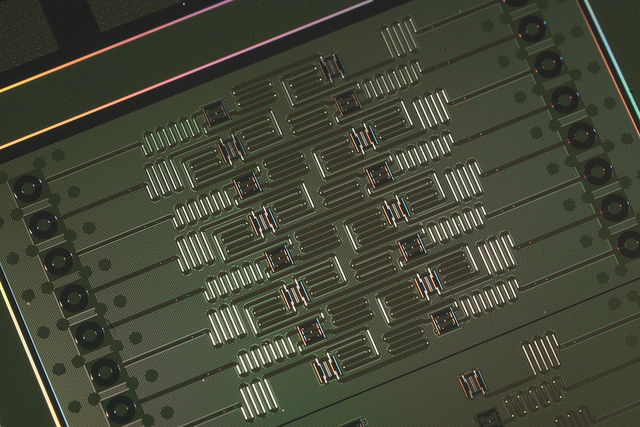
\includegraphics[width=4in]{review/ibmbuildsits.jpg}
                \caption{The IBM 16-qubit processor. Adapted from Ref.~\inlinecite{IBM16QubitsOriginal}.}
                \label{fig:ibmbuildsits}
            \end{figure}


After the increase in coherence time and the demonstration of basic algorithms and scalability, proposals and experiments turns to focus more on new architecture. One problem encountered when trying to scale up the superconducting qubit system is crossing of control, coupling and readout lines. Possible solutions require to go beyond the 2D structure, such as air bridge crossovers\cite{Versluis2016}, flip-chip\cite{Yorozu2006}, employing waveguide package resonance modes\cite{Minev2016} and using connected 3D cylindrical cavities\cite{Axline2016}. There are groups working on coupling superconducting qubits to flying qubits and mechanical resonators\cite{Palomaki2013,Reed2017,Keller2017}, aiming for the 6th and 7th DiVincenzo criteria.


% section history_of_the_development_of_transmon_qubit (end)


\section{Technical improvements} % (fold)
\label{sec:technical_improvements}

Much of the progress in the development of superconducting qubits came from clever design optimizations and technical improvements. The technical improvements can be roughly divided to several aspects including improving resonator quality factors, improving qubit control and measurement fidelity, and protecting qubits from decoherence.


Superconducting resonators were modeled and characterized in Ref.~\inlinecite{goppl2008coplanar}.


In summary, small junction is prefered to avoid defects. Removing loss from trapped vortices and quasiparticles by infrared and magnetic shielding is required for reliable resonator $Q$ measurement and for higher qubit coherence.

% section technical_improvements (end)










\chapter{微纳加工工艺} % (fold)
\label{cha:fabrication}

\section{光刻} % (fold)
\label{sec:光刻}
    \begin{enumerate}
        \item Spin coating S1805, 500 nm
        \begin{enumerate}
            \item 500rpm, 10s, 100rpm/s
            \item 4000rpm, 45s, 2000rpm/s
            \item 0rpm, 5s, 2000rpm/s
        \end{enumerate}
        \item Bake at 115 degree C for 1 min
        \item Align mask
        \item Expose with 405 nm UV light for 9.5s, power 350W
        \item Develop in MF-319 for 45s
        \item Clean in DI-water for 1min and blow dry
    \end{enumerate}
% section 光刻 (end)

\section{介电层生长与刻蚀} % (fold)
\label{sec:介电层生长与刻蚀}
    \begin{enumerate}
        \item PECVD生长SiO$_2$速率:70nm/min
        \item PECVD生长SiN$_x$速率:16nm/min
        \item ALD生长Al$_2$O$_3$速率:
        \item MF-319刻蚀Al$_2$O$_3$速率:
        \item MF-319刻蚀光刻胶速率:
        \item ICP刻蚀SiO$_2$速率:43.3nm/min
        \item ICP刻蚀SiN$_x$速率:50nm/min
    \end{enumerate}
    \subsection{刻蚀介电层后去除光刻胶} % (fold)
    \label{sub:刻蚀介电层后去除光刻胶}
        \begin{enumerate}
            \item 置于PG Remover中加热至85摄氏度,将烧杯口用铝箔纸盖住,保持85度30分钟
            \item 用丙酮,IPA清洗,氮气枪吹干
        \end{enumerate}
    % subsection 刻蚀介电层后的lift_off (end)
% section 介电层生长 (end)

\section{光刻胶Lift off} % (fold)
\label{sec:光刻胶lift_off}
        \begin{enumerate}
            \item 于NMP去胶液或丙酮中浸泡一晚,用铝箔纸盖住烧杯口
            \item 加热至85摄氏度15至30分钟,用铝箔纸盖住烧杯口
            \item 用镊子夹住片子后用胶头滴管于去胶液中吹洗
            \item 对于难以去除的区域,可尝试超声
            \item 对于生长了介电层后的器件,超声时应小心勿将介电层超声至脱落。对于30nm的SiO$_2$或30nm的SiN$_x$,可用60\% 功率,45kHz超声10秒,重复三次,即可去除对2.5维谐振腔样品可能出现的lift off不完全的情况,并保证介电层完整
            \item 目前尝试过用100\%功率,45kHz超声15秒,仍可保证介电层完整
            \item 从去胶液中取出后迅速放入丙酮中清洗,随后再放入IPA中清洗,最后用氮气枪吹干
        \end{enumerate}
    % section lift_off (end)

\section{磁控溅射镀膜} % (fold)
\label{sec:磁控溅射镀膜}
    \begin{enumerate}        
        \item Transfer to sputter chamber
        \item chamber -> Process
        \item open Ar valve, 100 sccm
        \item set DC parameter, I = 100mA
        \item DC -> on. If error, try with shutter open
        \item set I = 400mA
        \item set Ar to 6sccm
        \item set chrono end action to DC \& RF off and sputter shutters off
        \item Holder motion: Rotate
        \item open shutter and timing with chrono
        \item 25nm/min for sputtering Nb, hence 4min total time for 100nm Nb
        \item wait until end
        \item set Ar to 0sccm, close Ar valve
        \item Stop rotation, Chamber -> pump
        \item Holder motion -> transfer, start
        \item Transfer after pressure stable and chip cool
    \end{enumerate}
% section 磁控溅射镀膜 (end)

\section{Argon milling去除氧化层} % (fold)
\label{sec:argon_milling去除氧化层}


\begin{enumerate}
    \item transfer to oxid chamber
    \item Process-> IonGun
    \item Holder motion -> Target -> IonGun, start. Might error, start again
    \item Open Ar valve, set to 6sccm
    \item set Vbeam = 250V, Ibeam = 10mA, Vacc = 60V. Input parameters again even if they are already correct
    \item Discharge on, wait stable
    \item Beam on, wait 2min
    \item set Vbeam = 400V, Ibeam = 20mA, Discharge 40V, Vacc = 60V, Iacc = 1.1mA, wait stable
    \item ordinary status: pressure 1.2e-4Torr, cathode 7.1V, 6.22A, 40V/0.23A, 399V/20.1mA, 60V/1.1mA
    \item Set chrono end action to IonGun off
    \item open shutter and timing with chrono, 3min30s
    \item wait until end
    \item close shutter
    \item Ar off, Ar valve off
    \item oxid chamber -> pump
    \item Holder motions -> Transfer, start
    \item transfer after pressure stable
\end{enumerate}

% section argon_milling去除氧化层 (end)

\section{点焊} % (fold)
\label{sec:点焊}
    \begin{enumerate}
        \item 一焊由于PCB上的SMP接头的空间位置原因需位于器件上,二焊位于PCB板上,焊接使用铝线
        \item 一焊参数:功率220,时间30ms,力19
        \item 二焊参数:功率330,时间40ms,力19
        \item 点焊时应使焊线尽可能地短而密
    \end{enumerate}
% section 点焊 (end)
  

















% chapter fabrication (end)

\chapter{PPMS系统的常用操作} % (fold)
\label{cha:ppms系统的常用操作}
    对于PPMS的详细介绍可参阅PPMS的用户手册,本附录在读者熟悉PPMS相关术语与参数(如Chamber Pressure等)的前提下,为使用者提供一个方便参考的操作流程。

    在正常的测量状态下,Chamber Pressure与样品室温度有关,样品温度为2K左右时一般为300至400mTorr,chamber state应该为Purged,意为样品室已用He气清洗并抽真空。在非远程控制PPMS时,一般通过与PPMS相连的电脑上的MultiVu程序控制PPMS。该程序主面板下方有若干小面板,点击这些小面板可调出设定温度,磁场与样品室状态的分面板。常用的分面板也即前文提到的Temperature,Chamber,Field面板。

    \section{调节温度与磁场} % (fold)
    \label{sec:调节温度}
        在Temperature面板中,status显示当前样品温度。通过Control一栏即可设置目标温度(set point)以及调温的速率(Rate)。Mode选项有Fast settle和No overshoot两种,也即快速和非振荡的平稳到达目标温度两种模式。

        升温时最大速率不应超过20K/min,降温时最大速率不应超过10K/min。


        调节磁场与调节温度十分类似。
    % section 调节温度 (end)

    \section{更换样品} % (fold)
    \label{sec:更换样品}
        首先升温至室温,300K,从2K开始升温则需约30分钟。样品室升至常温后,样品室气压约为20~40Torr。点击Chamber分面板的Vent/Seal,此时样品室气压将快速升至常压,约790Torr,此后即可取出样品杆。若取出样品杆时间较长,应插入空样品杆并点击Chamber分面板的Purge/Seal以使样品室处于较好的密封环境。

        更换完样品并插入封好样品杆后,点击Chamber分面板的Purge/Seal,此时state变为Purging。样品室气压将在常压与~30Torr间来回反复若干次,约5分钟后state变为Purged,此时即可开始制冷。
    % section 更换样品 (end)
% chapter ppms系统的常用操作流程 (end)















\chapter{测量系统MATLAB代码} % (fold)
\label{cha:measurement_code}

通过MATLAB控制仪器,能够十分方便地调整仪器的各项参数以及从仪器采集所需数据。对于封装较好的代码,能够可扩展地编写与控制更为复杂的实验。因此我通过MATLAB实现了对VNA的控制与数据采集,基于PPMS仪器商提供的动态链接库文件实现了对PPMS系统的状态读取与控制。在这二者的基础上,编写了扫描不同温度与磁场下的频率响应的实验的代码。

本附录中将给出VNA与PPMS的MATLAB控制程序代码,以及扫描温度与磁场的MATLAB代码。


  \section{VNA控制代码} % (fold)
  \label{sec:vna控制代码}

  \begin{lstlisting}
classdef E5071C < handle
    % E5071C describe and control the agilent E5071C ENA
    %
    % EXAMPLES (assume instance named 'vna'):
    %   initialization:
    %       vna = E5071C;
    %       vna = E5071C('address',8,'InputBufferSize',100000);
    %   set & get parameters
    %       % fetch & return the start frequency:
    %       freq = vna.freqStart;
    %       % fetch & return the IFBW:
    %       bw = vna.ifbw;
    %       % set the stop frequency to 5GHz:
    %       vna.freqStop = 5e9;
    %       % set the number of average and turn on averaging:
    %       vna.avg = 999;
    %   fetch trace:
    %       % fetch the trace data, return a structure
    %       trace = vna.trace
    %
    %   See E5071C/plotTrace, E5071C/fit and E5071C/manualSweep for detail usage
    %
    %   Wentao, April 2017
    %
    
    properties (Constant)
        MAX_POINTS = 1601;
        MAX_AVG = 999;
        
    end

    properties
        visa
        InputBufferSize
        TimeOut
        
        address
        
        % properties with set & get methods
        freqStart
        freqStop
        freqSpan
        freqCenter        
        avg
        numOfPoints
        ifbw
        meas        
        outp
        power
        trigMode
        
        trace
        
        freqs
        h_fig       % figure handle
    end
    
    methods
        
        function obj = E5071C(varargin)
            % Initialize E5071C object
            %
            p = inputParser;
            p.addParameter('address',6, @isnumeric);        % GPIB address
            p.addParameter('InputBufferSize',30000, @isnumeric);
            p.addParameter('TimeOut',20, @isnumeric);
            p.parse(varargin{:});
            expandStructure(p.Results);
            
            obj.address = address;
            obj.TimeOut = TimeOut;
            obj.InputBufferSize = InputBufferSize;
            
            obj.visa = visa('agilent',sprintf('GPIB::%d::INSTR',obj.address));
            fprintf('%s\nConnected.\n',obj.read('*IDN?','%s'));
            set(obj.visa,'InputBufferSize', obj.InputBufferSize);
            set(obj.visa,'TimeOut', obj.TimeOut);
            % Set byte order to swapped (little-endian) format  
            fprintf('Set byte order to little-endian...');
            obj.write(':FORMAT:BORD SWAP');
            fprintf('Done.\n')
            % Set data type to real 64 bit binary block 
            fprintf('Set data type to real 64 bit binary block...');
            obj.write(':FORMAT:DATA REAL');
            fprintf('Done.\n');
        end
        
        function delete(obj)
            delete(obj.visa);
        end
        
        %% frequency set & get
        function value = get.freqStart(obj)
            value = obj.read(':sens:freq:star?', '%f');
        end
        function set.freqStart(obj,val)
            obj.write(':sens:freq:star %f',val);
        end
        function value = get.freqStop(obj)
            value = obj.read(':sens:freq:stop?', '%f');
        end
        function set.freqStop(obj,val)
            obj.write(':sens:freq:stop %f',val);
        end
        function value = get.freqCenter(obj)
            value = obj.read(':sens:freq:cent?', '%f');
        end
        function set.freqCenter(obj,val)
            obj.write(':sens:freq:cent %f',val);
        end
        function value = get.freqSpan(obj)
            value = obj.read(':sens:freq:span?','%f');
        end
        function set.freqSpan(obj,val)
            obj.write(':sens:freq:span %f', val);
        end
        
        %% sweep setup: measurement parameter, points, average, ifbw
        function value = get.meas(obj)
            value = obj.read(':CALC:PAR:DEF?', '%s');
        end
        function set.meas(obj, val)
            obj.write(':CALC:PAR:DEF %s', val);
        end
        function value = get.numOfPoints(obj)
            value = obj.read(':sens:swe:poin?', '%f');
        end
        function set.numOfPoints(obj, val)
            obj.write( ':sens:swe:poin %d', val);
        end
        
        function value = get.avg(obj)
            value = obj.read( ':sens:aver:count?', '%f');
        end
        function set.avg(obj, val)
            obj.write( ':sens:aver:count %d', val);
            obj.write(':SENSe:AVERage:STATe 1');
        end        
        function clearAvg(obj)
            obj.write(':SENSe:AVERage:CLE');
        end
        
        function value = get.ifbw(obj)
            value = obj.read(':sens:BWID:RES?', '%f');
        end
        function set.ifbw(obj, val)
            obj.write( ':sens:BWID:RES %f', val);
        end
        
        function val = sweepTime(obj)
            val = obj.read('SENS:SWE:TIME:DATA?','%f');
        end
        
        
        %% output & trigger
        function value = get.power(obj)
            value = obj.read(':SOURce:POWer:LEVel:IMMediate:AMPLitude?', '%f');
        end
        function set.power(obj, val)
            obj.write(':SOURce:POWer:LEVel:IMMediate:AMPLitude %d', val);
        end
        function value = get.outp(obj)
            value = obj.read(':OUTP:STATe?', '%f');
        end
        function set.outp(obj, val)
            obj.write(':OUTP:STATe %d', val);
        end
        function value = get.trigMode(obj)
            value = obj.read(':TRIG:SEQ:SOUR?','%s');
        end
        function set.trigMode(obj, val)
            % set.trigMode sets trigger mode
            %   available options: 'INT', 'EXT', 'MAN', 'BUS'
            %     Internal Trigger
            %     Uses the internal trigger to generate continuous triggers automatically.
            % 
            %     External Trigger
            %     Generates a trigger when the trigger signal is inputted externally via the Ext Trig connector or the handler interface.
            % 
            %     Manual Trigger
            %     Generates a trigger when the key operation of Trigger > Trigger is executed from the front panel.
            % 
            %     Bus Trigger
            %     Generates a trigger when the SCPI.IEEE4882.TRG object is executed.

            obj.write(':TRIG:SEQ:SOUR %s',val);
        end
        
        %% set & get configurations
        function setConfig(obj, config)
            % setConfig apply parameters to E5071C
            % config should have same or less fields as E5071C properties
            % with set & get methods
            flds = fieldnames(config);
            for ii = 1:length(flds)
                fld = flds{ii};
                obj.(fld) = config.(fld);
            end
        end
        
        function params = getConfig(obj)
            % getConfig returns E5071C object parameters for saving
            % configuration
            flds = {'freqStart',...
                'freqStop',...
                'freqSpan',...
                'freqCenter',...
                'avg',...
                'numOfPoints',...
                'ifbw',...
                'meas',...
                'outp',...
                'power',...
                'trigMode'};            
            for ii = 1:length(flds)
                fld = flds{ii};
                params.(fld) = obj.(fld);
            end
        end
        
        
        %% get & plot trace
        function autoScale(obj)
            % autoScale auto-scales the y axis
            % for viewing the image via web server
            obj.write(':DISP:WIND:TRAC:Y:SCAL:AUTO');
        end
        function value = get.freqs(obj)            
            value = obj.freqStart:((obj.freqStop...
                - obj.freqStart)/obj.numOfPoints):obj.freqStop;
            value = value(1:end-1);
        end
        function value = get.trace(obj)
            % adopted from https://community.keysight.com/thread/22342
            fopen(obj.visa);
            fprintf(obj.visa, 'CALC:DATA:SDAT?'); 
            [data, count, msg] = binblockread(obj.visa, 'double'); 
            fclose(obj.visa);
            value.count = count;
            value.msg = msg;
            value.X = data(1:2:end); 
            value.Y = data(2:2:end);
        end
        
        function titleStr = plotTrace(obj, varargin)
            % plotTrace fetch & plot trace data
            % EXAMPLE (assume the object is named 'vna'):
            %   vna.plotTrace;
            %   vna.plotTrace('issavefig', true);
            %   vna.plotTrace('issavefig', true,'filename','test');
            %
            % See the inputParser below for more options
            %   
            
            p = inputParser;
            p.addParameter('issavedata',false,@islogical);
            p.addParameter('issavefig',false,@islogical);
            p.addParameter('avg',1,@isnumeric);
            p.addParameter('filename','',@ischar);
            p.addParameter('format','png',@ischar);
            p.parse(varargin{:});
            expandStructure(p.Results);
            
            if avg > 1
                pause(round(avg*obj.sweepTime + 1));
            end
            
            hfig = figure;
            obj.h_fig = hfig;
            trace = obj.trace;
            
            plot(obj.freqs/1e9,...
                20*log10(abs(trace.X + 1i*trace.Y)));
            xlabel freq/GHz
            ylabel SParameter/dB
            titleStr = ['start_' num2str(obj.freqStart/1e9)...
                'GHz_stop_'  num2str(obj.freqStop/1e9)...
                'GHz_pow_' num2str(obj.power)...
                'dBm_AVG_' num2str(avg)];
            title(titleStr, 'interpreter','none');
            
            if issavefig
                if ~isempty(filename)
                    titleStr = filename;
                end
                saveas(hfig, [titleStr format]);
            end
            
            if issavedata  
                str = titleStr;
                freqs = obj.freqs;
                config = obj.getConfig;
                save([str '.mat'],'freqs','trace','str','config');
            end      
            
        end
        
        function [freqs, trace] = manualSweep(obj, varargin)
            % manualSweep defines and does a manual frequency sweep
            % main purpose is for wide sweep with high resolution for
            % finding modes
            %
            % EXAMPLE:
            %   [freqs, trace] = vna.manualSweep('start',1e9,'stop',9e9,'res',1e5);
            %   [freqs, trace] = vna.manualSweep('start',3.5e9,'stop',3.6e9,'res',1e4, 'avg',999);
            %   [freqs, trace] = vna.manualSweep('center',4.9655e9,'span',1e6,'res',0.001e6,'avg',2,'ifbw',100,'pow',-10);
            %
            %
            % See the inputParser below for more options
            %
            
            p = inputParser;
            p.addParameter('start',1e9,@isnumeric); % start frequency
            p.addParameter('stop',8e9,@isnumeric);  % stop frequency
            p.addParameter('res',1e6,@isnumeric);   % frequency resolution
            p.addParameter('avg', 1, @isnumeric);       % number of average
            p.addParameter('ifbw', 100, @isnumeric);    % ifbw of vna
            p.addParameter('points', obj.MAX_POINTS, @isnumeric); % number of points of vna
            p.addParameter('pow', -100, @isnumeric); % power of vna, default below
                                                        % the lowest power of E5071C,
                                                        % hence this
                                                        % parameter only
                                                        % takes effect if it
                                                        % is given a valid
                                                        % value
            p.addParameter('center', 0, @isnumeric);  % frequency sweep can also be defined
                                                      % by center and span,
                                                      % if they are given a
                                                      % valid value
            p.addParameter('span',0, @isnumeric);
            p.addParameter('issavedata',true,@islogical);
            p.addParameter('hfig',233,@isnumeric);      % figure handle
            p.addParameter('notes','',@ischar);         % notes to add in file name
            
            p.parse(varargin{:});
            expandStructure(p.Results);
            
            freqSectionSpan = res * points;
            freqSectionSpan = 1e6 * round(freqSectionSpan/1e6);
            if span ~= 0 && center ~= 0
                start = center - span/2;
                stop = center + span/2;
            end
            numOfSections = ceil((stop - start)/freqSectionSpan);
            stop = start + numOfSections * freqSectionSpan;
            totalPoints = points * numOfSections;
            
            % initialize
            freqs = NaN(1, totalPoints);
            trace.X = freqs;
            trace.Y = freqs;
            
            % apply parameters
            obj.ifbw = ifbw;
            if pow > -85
                obj.power = pow;
            end
            obj.numOfPoints = points;
            obj.freqSpan = freqSectionSpan;
            obj.avg = obj.MAX_AVG;
            
            sweepTime = obj.sweepTime;
            waitTime = ceil(avg * sweepTime) + 1;
            
            figure(hfig);
            xlabel freq/GHz
            ylabel SParameter/dB
            str = sprintf('start_%.2fGHz_stop_%.2fGHz_res_%.2fMHz_pow_%ddBm_AVG_%d',...
                start/1e9,stop/1e9,res/1e6,obj.power,avg);
            title(str,'interpreter','none');
            
            fprintf('\tsweep from %.2fGHz to %.2fGHz, %d sections, %ds per section\n\ttotal points: %d, total time: %ds.\n',...
                start/1e9,stop/1e9, numOfSections,waitTime,totalPoints, waitTime * numOfSections);
            for i = 1:numOfSections
                obj.freqCenter = start + freqSectionSpan/2 +  freqSectionSpan* (i-1);
                fprintf('sweeping %.2fGHz to %.2fGHz...\n',obj.freqStart/1e9,obj.freqStop/1e9);
                pause(waitTime);
                tmptrace = obj.trace;
                tmpfreqs = obj.freqs;
                freqs((1 + (i-1)*points):(i*points)) = tmpfreqs;
                trace.X((1 + (i-1)*points):(i*points)) = tmptrace.X';
                trace.Y((1 + (i-1)*points):(i*points)) = tmptrace.Y';
                figure(hfig);
                plot(freqs/1e9, 20*log10(abs(trace.X + 1i*trace.Y)));
            end
            fprintf('Sweep finished!\n');
            
            figure(hfig);
            xlabel freq/GHz
            ylabel SParameter/dB
            str = sprintf('start_%.2fGHz_stop_%.2fGHz_res_%.2fMHz_pow_%ddBm_AVG_%d%s',...
                start/1e9,stop/1e9,res/1e6,pow,avg,notes);
            title(str,'interpreter','none');
            
            if issavedata
                config = obj.getConfig;
                save([str '.mat'],'freqs','trace','str','config');
            end      
            obj.h_fig = hfig;
            
        end
        
        
        
        function [freqs,totalWaitTime] = manualSweepFreqs(obj, varargin)
            % manualSweepFreqs quickly calculate frequencies of
            % manualSweep, does not do the sweep
            %
            % ATTENTION: this method will modify the vna sweep frequency!
            %
            % See the inputParser below for more options
            %
            
            p = inputParser;
            p.addParameter('start',1e9,@isnumeric); % start frequency
            p.addParameter('stop',8e9,@isnumeric);  % stop frequency
            p.addParameter('res',1e6,@isnumeric);   % frequency resolution
            p.addParameter('avg', 1, @isnumeric);       % number of average
            p.addParameter('ifbw', 100, @isnumeric);    % ifbw of vna
            p.addParameter('points', obj.MAX_POINTS, @isnumeric); % number of points of vna
            p.addParameter('pow', -100, @isnumeric); % power of vna, default below
                                                        % the lowest power of E5071C,
                                                        % hence this
                                                        % parameter only
                                                        % takes effect if it
                                                        % is given a valid
                                                        % value
            p.addParameter('center', 0, @isnumeric);  % frequency sweep can also be defined
                                                      % by center and span,
                                                      % if they are given a
                                                      % valid value
            p.addParameter('span',0, @isnumeric);
            
            % useless, but required for input parser to be identical with input parser for manualSweep; 
            p.addParameter('issavedata',true,@islogical);
            p.addParameter('hfig',233,@isnumeric);      % figure handle
            p.addParameter('notes','',@ischar);         % notes to add in file name
            
            
            p.parse(varargin{:});
            expandStructure(p.Results);
            
            freqSectionSpan = res * points;
            freqSectionSpan = 1e6 * round(freqSectionSpan/1e6);
            if span ~= 0 && center ~= 0
                start = center - span/2;
                stop = center + span/2;
            end
            numOfSections = ceil((stop - start)/freqSectionSpan);
            stop = start + numOfSections * freqSectionSpan;
            totalPoints = points * numOfSections;
            
            % initialize
            freqs = NaN(1, totalPoints);
            
            % apply parameters
            obj.ifbw = ifbw;
            if pow > -85
                obj.power = pow;
            end
            obj.numOfPoints = points;
            obj.freqSpan = freqSectionSpan;
            obj.avg = obj.MAX_AVG;
            
            sweepTime = obj.sweepTime;
            waitTime = ceil(avg * sweepTime) + 1;
            totalWaitTime = waitTime * numOfSections;
            
            for i = 1:numOfSections
                obj.freqCenter = start + freqSectionSpan/2 +  freqSectionSpan* (i-1);

                tmpfreqs = obj.freqs;
                freqs((1 + (i-1)*points):(i*points)) = tmpfreqs;
            end
            
        end
      
        %% fit
        function  [ f_r,Q_i,Q_c,Q_l ] = fit(obj,varargin)
            % select range and fit plot
            % ATTENTION: use vna.plotTrace or vna.manualSweep first and then use vna.fit!
            % EXAMPLE:
            %   vna.plotTrace;
            %   vna.fit('fitall',true);
            % you can also give data to this method:            
            %     [ f_r,Q_i,Q_c,Q_l ] = vna.fit('fitall',true,'issavefig',false,...
            %                                   'xdata',freqs,'ydata',20*log10(abs(SParams)),...
            %                                   'titleNotes','_pow_-10dBm' );
            %
            % See the inputParser below for more options
            %
            
            p = inputParser;
            p.addParameter('issavefig',true,@islogical);% if true, save fig to png file
            p.addParameter('fitall', false,@islogical); % if true, fit all
                                                        % plotted data,
                                                        % else ask two
                                                        % input for the fit
                                                        % range
            p.addParameter('xdata',[],@isnumeric);      % xdata in GHz frequency
            p.addParameter('ydata',[],@isnumeric);      % ydata given in dB
            p.addParameter('titleNotes','',@ischar);    % notes to add to the figure title
            p.addParameter('QGuess',1e5,@isnumeric);
            p.parse(varargin{:});
            expandStructure(p.Results);
            
            dataObj = get(gca,'children');
            if isempty(xdata)
                xdata = get(dataObj,'xdata');
            end
            if isempty(ydata)
                ydata = get(dataObj,'ydata');
            end
            
            if gcf == obj.h_fig
                figure(obj.h_fig);
            else
                figure(obj.h_fig);
                plot(xdata, ydata);
                % assume GHz frequency
                xlabel frequency/GHz;
                ylabel S/dB;
                title([sprintf('start_%.4fGHz_stop_%.4fGHz',...
                    min(xdata)/1e9, max(xdata)/1e9 ) titleNotes],'interpreter','none');
            end
                
            if fitall
                leftInd = 1;
                rightInd = length(xdata);
            else
                fprintf('Select the X range for fitting:');
                tmpPoints = ginput(2);
                leftX = min(tmpPoints(:,1));
                rightX = max(tmpPoints(:,1));
                leftInd = find(leftX < xdata, 1);
                rightInd = find(rightX < xdata, 1);
            end
            t = xdata(:);
            y = ydata(:);
            % assume xdata given in GHz
            t = t(leftInd:rightInd)*1e9;
            % assume ydata given in dB, convert to linear
            y = 10.^(y(leftInd:rightInd)./20);

            % guess initial parameters
            peakInd = find(abs(ydata)>=max(abs(ydata)),1);
            freq0 = xdata(peakInd); % in GHz
            x1 = [freq0, QGuess/1e4, QGuess/1e4, 0, 0, 0];

            % fit with complex S21 deduced theoretically
            % 8 parameter, linear base
            %         F = @(x,xdata)(20.*log10(abs(x(6).*(1+x(5).*(xdata-x(1).*1e9)./(x(1).*1e9)).*(1-(x(2).^2.*1e4.*x(3).^2.*1e4./cos(x(4)))./(x(2).^2.*1e4 + x(3).^2.*1e4./cos(x(4)))./(x(3).^2.*1e4).*(cos(x(4))+1i.*sin(x(4)))./(1+2.*1i.*(x(2).^2.*1e4.*x(3).^2.*1e4./cos(x(4)))./(x(2).^2.*1e4 + x(3).^2.*1e4./cos(x(4))).*(xdata-x(1).*1e9)./(x(1).*1e9)))))+x(7).*xdata.*1e-9+x(8));
            % 7 parameter, constant base
            F = @(x,xdata)(abs(x(6).*(1+x(5).*(xdata-x(1).*1e9)./(x(1).*1e9)).*(1-(x(2).^2.*1e4.*x(3).^2.*1e4./cos(x(4)))./(x(2).^2.*1e4 + x(3).^2.*1e4./cos(x(4)))./(x(3).^2.*1e4).*(cos(x(4))+1i.*sin(x(4)))./(1+2.*1i.*(x(2).^2.*1e4.*x(3).^2.*1e4./cos(x(4)))./(x(2).^2.*1e4 + x(3).^2.*1e4./cos(x(4))).*(xdata-x(1).*1e9)./(x(1).*1e9)))));
            %x(1): f, center frequency, in GHz
            %x(2): Qi, intrinsic Q, Ql = Qi*Qc/(Qi + Qc) =  (x(2).*x(3)./cos(x(4)))./(x(2) + x(3)./cos(x(4))), in 1e4
            %x(3): |Qe|, parameter Q, 1/Qc = Re (1/Qe) = cos(theta)/Qe, in 1e4
            %x(4): theta, phase of parameter Q
            %x(5): alpha
            %x(6): amplitude A

    
            opt=optimset('MaxIter',10000,'MaxFunEvals',10000,'tolx',1e-16,'tolf',1e-9);
            for loop_fit=1:5            
                [x_fit1,resnorm,~,exitflag,output] = lsqcurvefit(F,x1,t,y,[],[],opt);
                x1=x_fit1;
                if ((x1(4)>pi/2)||(x1(4)<-pi/2))
                    tmp = floor(abs(x1(4))./(pi/2));
                    if x1(4)>0
                        x1(4)=x1(4)-tmp.*pi/2;
                    end
                    if x1(4)<0
                        x1(4)=x1(4)+tmp.*pi/2;
                    end
                end
            end
            
            f_r = x1(1)*1e9; % center frequency, in Hz
            Q_i = x1(2).^2.*1e4; % interal Q
            Q_c = x1(3).^2./cos(x1(4)).*1e4;  % coupled Q
            Q_l = Q_i.*Q_c./(Q_i + Q_c);  % loaded Q
            
            figure(obj.h_fig);
            hold on
            plot(t/1E9,20*log10(y),'.',t/1E9,20*log10(F(x_fit1,t)),'LineWidth',2);
            f_text=['f_r = '];
            f_text=[f_text num2str(f_r/1e9)];
            f_text=[f_text 'GHz'];
            Ql_text=['Q_l = ' num2str(round(Q_l))];
            Qi_text=['Q_i = ' num2str(round(Q_i))];
            Qc_text=['Q_c = ' num2str(round(Q_c))];
            text_pos=[(max(20*log10(y))-min(20*log10(y)))/4+min(20*log10(y)),min(20*log10(y))];
            text(t(1)/1E9,text_pos(1),f_text,'FontSize',18);
            text(t(1)/1E9,text_pos(2),Ql_text,'FontSize',18);
            text(t(round(end/1.5))/1E9,text_pos(1),Qi_text,'FontSize',18);
            text(t(round(end/1.5))/1E9,text_pos(2),Qc_text,'FontSize',18);
            hold off
            
            if issavefig
                str = ['Fit_' get(get(gca,'Title'),'String') '.png'];
                saveas(obj.h_fig,str);   
                fprintf(['Image ' str ' saved.\n'])
            end

        end
        
        
    end
    
        
    
    %% private methods
    methods (Access = private)
        function val = read(obj, varargin)
            % varargin{1:(end-1)} are commands to be sent as a formatted
            % string
            % varargin{end} is the read format
            fopen(obj.visa);
            fprintf(obj.visa, varargin{1:(end-1)});
            val = fscanf(obj.visa, varargin{end});
            fclose(obj.visa);
        end
        function write(obj, varargin)
            fopen(obj.visa);
            fprintf(obj.visa, varargin{:});
            fclose(obj.visa);
        end
    end
end
  \end{lstlisting}
    
  % section vna控制代码 (end)

  \section{PPMS控制代码} % (fold)
  \label{sec:ppms控制代码}
  \begin{lstlisting}
classdef PPMS < handle
    % PPMS describe and control QDInstrument DynaCool at IIIS via QDInstrument.dll,
    % which is much faster than using dll created from LabVIEW.
    %
    % Calling dll created from LabVIEW is slow and generates new client
    % at each function call, which is very bad and troublesome. This
    % version of PPMS avoided the above two problems.
    %
    % EXAMPLES (assuming instance named 'ppms'):
    %
    % Initialization:
    %   ppms = PPMS;
    %   ppms = PPMS('address','101.6.98.151','isremote',true,'dllfilepath','C:\Users\IIIS\Documents\MATLAB\PPMS\QDInstrument.dll');
    % Get temperature value and status:
    %   temp = ppms.temp;
    %   stat = ppms.tempStatus;     % This returns a .NET object, use
    %                               % char(stat.ToString) to get the
    %                               % string, or directly use char(ToString(ppms.fieldStatus))
    %   statStr = ppms.tempStatusStr;   % Directly get the temperature
    %                                   % status string
    % Get field value and status:
    %   fld = ppms.field;
    %   stat = ppms.fieldStatus;    % See notes for ppms.tempStatus above
    %   statStr = ppms.fieldStatusStr;  % Directly get the field
    %                                   % status string
    %
    % Set temperature:
    %   ppms.setTemp(4);
    %   ppms.setTemp(2,'tempRate',5,'tempApproach','NoOvershoot');
    %   ppms.setTemp(300,'tempRate',20,'tempApproach','FastSettle');
    %
    % Set field, field strength in Gauss (Oe):
    %   ppms.setField(0,'fieldRate',50,'fieldApproach','Linear');
    %   ppms.setField(200,'fieldRate',100);
    %   ppms.setField(500,'fieldMode','Persistent');
    % 
    % See Constant properties for available options for 'tempApproach',
    % 'fieldApproach', and 'fieldMode'
    %
    % ATTENTION: 
    %   1. Setting 'fieldMode' to 'Persistent' etc. is not working as
    %       expected.
    %   2. Sometimes you might need to manually load the dll file using NET.addAssembly(dllfilepath)
    %       when you first started MATLAB, try initializing ppms and also try
    %       calling QuantumDesign.QDInstrument.QDInstrumentType.DynaCool
    %       etc. for multiple times until it works. It will work when
    %       auto-completion (by using TAB button) works.
    %
    % In development (May 12, 2017)
    % Testing (May 13, 2017)
    % Add get status in string format (May 14, 2017)
    % Wentao, May 2017
    %

properties (Constant)
    % the second argument (numeric arrays) of these Constants is of no use
    % the containers.Map is used for utilizing the isKey method, see
    % the prirvate methods for parameter verification.
    INSTR_TYPE = containers.Map({'PPMS','VersaLab','DynaCool','SVSM'},[0,1,2,3]);
    
    TEMP_APPROACH = containers.Map({'FastSettle','NoOvershoot'},[0,1]);
    
    FIELD_APPROACH = containers.Map({'Linear','NoOvershoot','Oscillate'},...
                        [0,1,2]);
    FIELD_MODE = containers.Map({'Persistent','Driven'},[0,1]);
    
end

properties
    dllfilepath
    address
    isremote
    instrType
    
    QDInstr
    vi
    
    temp
    field
    tempStatus
    fieldStatus
    
    tempApproach
    tempRate
    fieldMode
    fieldRate
    fieldApproach
end

methods
    function obj = PPMS(varargin)
        % initialize PPMS
        p = inputParser;
        p.addParameter('address','101.6.98.151',@ischar);       % ip address of PPMS computer
        p.addParameter('dllfilepath','C:\Users\IIIS\Documents\MATLAB\PPMS\QDInstrument.dll',@ischar);
        p.addParameter('isremote',true,@islogical);             % is remote (is MATLAB and MultiVu on different computer)
        p.addParameter('instrType','DynaCool',@checkInstrType); % instrument type
        
        p.parse(varargin{:})
        expandStructure(p.Results);
        
        
        obj.address = address;
        obj.dllfilepath = dllfilepath;
        obj.isremote = isremote;
        obj.instrType = instrType;
        obj.tempApproach = 'Unknown';
        obj.fieldMode = 'Unknown';
        obj.fieldApproach = 'Unknown';
        obj.tempRate = NaN;
        obj.fieldRate = NaN;
        
        obj.QDInstr = NET.addAssembly(dllfilepath);
        pause(1);
        obj.tempStatus = QuantumDesign.QDInstrument.TemperatureStatus.TemperatureUnknown;
        obj.fieldStatus = QuantumDesign.QDInstrument.FieldStatus.MagnetUnknown;
        
        % initialize .NET object which is the vi for the ppms
        obj.vi = QuantumDesign.QDInstrument.QDInstrumentFactory.GetQDInstrument(...
                            QuantumDesign.QDInstrument.QDInstrumentType.(instrType),...
                            isremote,address,uint16(11000) );
        fprintf('PPMS %s at %s connected.\n',obj.instrType, obj.address);
        
        
    end
    
    %% set & get temperature
    function value = get.temp(obj)
        [~, value, obj.tempStatus] = GetTemperature(obj.vi, double(0), obj.tempStatus);
    end
    function value = get.tempStatus(obj)
        [~, obj.temp, value] = GetTemperature(obj.vi, double(0), obj.tempStatus);
    end
    function str = tempStatusStr(obj)
        str = char(ToString(obj.tempStatus));
    end
    
    function setTemp(obj,varargin)
        p = inputParser;
        p.addRequired('temperature');
        p.addParameter('tempRate',10,@isnumeric);
        p.addParameter('tempApproach','FastSettle',@obj.checkTempApproach);
        p.parse(varargin{:});
        expandStructure(p.Results);
        
        obj.tempApproach = tempApproach;
        obj.tempRate = tempRate;
        
        SetTemperature(obj.vi, double(temperature),double(tempRate),...
                        QuantumDesign.QDInstrument.TemperatureApproach.(tempApproach));     
        
        
    end
    
    
    %% set & get field
    function value = get.field(obj)
        [~, value, obj.fieldStatus] = GetField(obj.vi, 0, obj.fieldStatus);
    end
    function value = get.fieldStatus(obj)
        [~, obj.field, value] = GetField(obj.vi, 0, obj.fieldStatus);
    end
    function str = fieldStatusStr(obj)
        str = char(ToString(obj.fieldStatus));
    end
    
    function setField(obj,varargin)
        p = inputParser;
        p.addRequired('b_field');
        p.addParameter('fieldRate',100,@isnumeric);
        p.addParameter('fieldMode','Driven',@obj.checkFieldMode)
        p.addParameter('fieldApproach','Linear',@obj.checkFieldApproach);
        p.parse(varargin{:});
        expandStructure(p.Results);
        
        obj.fieldMode = fieldMode;
        obj.fieldRate = fieldRate;
        obj.fieldApproach = fieldApproach;
        
        SetField(obj.vi, double(b_field),double(fieldRate),...
                        QuantumDesign.QDInstrument.FieldApproach.(fieldApproach),...
                        QuantumDesign.QDInstrument.FieldMode.(fieldMode));         
        
    end
    
    %% TODO: add set & get chamber (not so necessary since we have remote desktop)
    
    %% quick methods
    function warmup(obj)
        obj.setField(0);
        obj.setTemp(300,'tempRate',20);
    end
    
    
end

methods(Access = private)
    % methods for checking string input validity
    function passed = checkInstrType(obj, instrType)
        passed = isKey(obj.INSTR_TYPE, instrType);
    end

    function passed = checkTempApproach(obj, tempMode)
        passed = isKey(obj.TEMP_APPROACH,tempMode);
    end
    
    function passed = checkFieldMode(obj, fieldMode)
        passed = isKey(obj.FIELD_MODE,fieldMode);
    end
    function passed = checkFieldApproach(obj, fieldApproach)
        passed = isKey(obj.FIELD_APPROACH,fieldApproach);
    end
end
end
  \end{lstlisting}
    
  % section ppms控制代码 (end)

  \section{扫描温度与磁场实验的代码} % (fold)
  \label{sec:扫描温度与磁场实验的代码}
  \subsection{扫描温度} % (fold)
  \label{sub:扫描温度}
\begin{lstlisting}
%%
function [tempStableTmr, setTempTmr] = TempSweep(ppms,vna,temps,varargin)
% temperature sweep
%
% Parameters:
%   ppms: the PPMS object
%   vna: the E5071C object
%   temps: temperatures to sweep
%   varargin: optional input arguments, see inputParser below for detail
%
% Returns:
%   Two timer object tempStableTmr and setTempTmr.
% 
%   Sweep results will be automatically saved.
%   You can also find parameters and sweep results in
%   tempStableTmr.UserData and setTempTmr.UserData
%   It's better to delete and clear the timer object since they'll remained
%   in the memory:
%         delete(tempStableTmr);
%         delete(setTempTmr);
%         clear setTempTmr;
%         clear tempStableTmr;
%
% ATTENTION: the waiting process (for the temperature to be stable) is 
% going in the background, when you can do stuff in the command line at
% the same time. HOWEVER, the vna sweep is not and the command line 
% won't react during the vna sweep.
%
% In development (May 13, 2017)
% 
% TODO: 
%   Done. add input parser
%   Done. choose vna sweep mode. Change 'plotTrace' to 'fetchTrace'
%   Done. choose temperature wait mode ('Near' or 'Stable')
%   Done. fetch actual temperatures and add timeStamps;
% 
% Wentao, May 2017
%

p = inputParser;
p.addParameter('vnaMode','plotTrace',@ischar);      % fetchTrace will directly fetch vna trace.
                                                    % Else, the E5071C/manualSweep method is called
p.addParameter('checkTempPeriod',10,@isnumeric);
p.addParameter('tempWaitMode','Stable',@ischar);    % another option is 'Near'
p.addParameter('manualSweepConfig',struct([]),@isstruct);   % parameters for the E5071C/manualSweep method as a structure

p.parse(varargin{:});
expandStructure(p.Results);

if strcmpi(vnaMode, 'plotTrace')
    freqs = vna.freqs;
    waitTime = vna.sweepTime;
else
    [freqs,waitTime] = vna.manualSweepFreqs(manualSweepConfig);
end
tempStableTmr = timer;
setTempTmr = timer;
set(tempStableTmr,'ExecutionMode','fixedRate');
set(tempStableTmr,'period',checkTempPeriod);    % check temperature stable period
set(tempStableTmr,'TimerFcn',@timerCalled);
set(tempStableTmr,'userdata',struct('ppms',ppms,'numOfTemps',length(temps),...
                            'manualSweepConfig',manualSweepConfig,...
                            'tempWaitMode',tempWaitMode,...
                            'vnaMode',vnaMode,...
                            'freqs',freqs,...
                            'timeStamps',NaN(1,length(temps)),...
                            'actualTemps',NaN(1,length(temps)),...
                            'vna',vna,'t',setTempTmr,'waitTime',waitTime,...
                            'cnt',1,'SParams',NaN(length(temps),length(freqs)) ) );

set(setTempTmr,'userdata',struct('ppms',ppms,'t',tempStableTmr,'temps',temps,'cnt',1) );
set(setTempTmr,'TimerFcn',@setTempTimerCalled);

start(setTempTmr);
end

%%
function timerCalled(thisObj,event)
ud = thisObj.UserData;
expandStructure(ud);
stat = char(ToString(ppms.tempStatus));
if strcmpi(stat, tempWaitMode)
    fprintf('Temperature %s, start vna averaging (%.2fs)...\n',...
            tempWaitMode,waitTime+0.5)
    
    % vna sweep
    if strcmpi(vnaMode, 'plotTrace')
        vna.clearAvg;
        pause(waitTime+0.5);
        trace = vna.trace;
    else
        [~,trace] = vna.manualSweep(manualSweepConfig);
    end
    fprintf('vna trace fetched.\n');
    
    % save SParams back into timer
    ud.actualTemps(cnt) = ppms.temp;
    ud.timeStamps(cnt) = now;
    ud.SParams(cnt,:) = trace.X(:)' + 1i*trace.Y(:)';
    ud.cnt = cnt + 1;
    thisObj.UserData = ud;
    stop(thisObj);
    fprintf('Temperature timer stopped at %s.\n', datestr(now,30))
    if ud.cnt <= numOfTemps
        fprintf('\n');
        start(t);
    else
        fprintf('Temperature sweep finished at %s\n',datestr(now,30));
        % save data
        expandStructure(ud);
        ud2 = t.UserData;
        setTemps = ud2.temps;
        actualTemps = ud.actualTemps;
        timeStamps = ud.timeStamps;
        startF = min(ud.freqs);
        stopF = max(ud.freqs);
        pow = vna.power;
        config = vna.getConfig;
        minT = min(setTemps);
        maxT = max(setTemps);
        fname = sprintf('TempSweep_start_%.4fGHz_stop_%.4fGHz_pow_%.1fdBm_minT_%.3fK_maxT_%.3fK_numT_%d_%s.mat',...
            startF/1e9,stopF/1e9,pow,minT,maxT,length(setTemps),datestr(now,30));
        save(fname,'SParams','waitTime','setTemps','actualTemps',...
            'freqs','config','timeStamps','manualSweepConfig');
        fprintf('%s saved.\n',fname);
    end
else
    fprintf('Temperature is %s. Waiting for temperature to be %s...\n',...
        stat,tempWaitMode)
end

end

%%
function setTempTimerCalled(thisObj,event)
ud = thisObj.UserData;
expandStructure(ud);
temp = temps(cnt);
fprintf('Set ppms temperature to %.4f K, %s\n',temp,datestr(now,30));
ppms.setTemp(temp,'tempApproach','NoOvershoot','tempRate',1);
pause(0.5);
start(t);
ud.cnt = cnt+1;
thisObj.UserData = ud;

end
\end{lstlisting}
  % subsection 扫描温度 (end)

  \subsection{扫描磁场} % (fold)
  \label{sub:扫描磁场}
  \begin{lstlisting}
%%
function [fldStableTmr, setFldTmr] = FieldSweep(ppms,vna,BFields,varargin)
% field sweep
%
% Parameters:
%   ppms: the PPMS object
%   vna: the E5071C object
%   BFields: Magnetic fields to sweep, in ***GAUSS***!!! (1 gauss = 0.1 mT)
%   varargin: optional input arguments, see inputParser below for detail
%
% Returns:
%   Two timer object tempStableTmr and setTempTmr.
% 
%   Sweep results will be automatically saved.
%   You can also find parameters and sweep results in
%   fldStableTmr.UserData and setFldTmr.UserData
%   It's better to delete and clear the timer object since they'll remained
%   in the memory:
%         delete(fldStableTmr);
%         delete(setFldTmr);
%         clear fldStableTmr;
%         clear setFldTmr;
%
% ATTENTION: the waiting process (for the field to be stable) is 
% going in the background, when you can do stuff in the command line at
% the same time. HOWEVER, the vna sweep is not and the command line 
% won't react during the vna sweep.
%
% In development (May 16, 2017)
% 
% Wentao, May 2017
%

p = inputParser;
p.addParameter('vnaMode','plotTrace',@ischar);      % fetchTrace will directly fetch vna trace.
                                                    % Else, the E5071C/manualSweep method is called
p.addParameter('checkFldPeriod',5,@isnumeric);
p.addParameter('fldWaitMode','StableDriven',@ischar);    % another option is 'Near'
p.addParameter('manualSweepConfig',struct([]),@isstruct);   % parameters for the E5071C/manualSweep method as a structure

p.parse(varargin{:});
expandStructure(p.Results);

if strcmpi(vnaMode, 'plotTrace')
    freqs = vna.freqs;
    waitTime = vna.sweepTime;
else
    [freqs,waitTime] = vna.manualSweepFreqs(manualSweepConfig);
end
fldStableTmr = timer;
setFldTmr = timer;
set(fldStableTmr,'ExecutionMode','fixedRate');
set(fldStableTmr,'period',checkFldPeriod);    % check field stable period
set(fldStableTmr,'TimerFcn',@timerCalled);
set(fldStableTmr,'userdata',struct('ppms',ppms,'numOfFlds',length(BFields),...
                            'manualSweepConfig',manualSweepConfig,...
                            'fldWaitMode',fldWaitMode,...
                            'vnaMode',vnaMode,...
                            'freqs',freqs,...
                            'timeStamps',NaN(1,length(BFields)),...
                            'actualFields',NaN(1,length(BFields)),...
                            'vna',vna,'t',setFldTmr,'waitTime',waitTime,...
                            'cnt',1,'SParams',NaN(length(BFields),length(freqs)) ) );

set(setFldTmr,'userdata',struct('ppms',ppms,'t',fldStableTmr,...
                                'BFields',BFields,'cnt',1) );
set(setFldTmr,'TimerFcn',@setFldTimerCalled);

start(setFldTmr);
end

%%
function timerCalled(thisObj,event)
ud = thisObj.UserData;
expandStructure(ud);
stat = char(ToString(ppms.fieldStatus));
if strcmpi(stat, fldWaitMode)
    fprintf('Field %s, start vna averaging (%.2fs)...\n',...
            fldWaitMode,waitTime+0.1)
    
    % vna sweep
    if strcmpi(vnaMode, 'plotTrace')
        vna.clearAvg;
        pause(waitTime+0.1);
        trace = vna.trace;
    else
        [~,trace] = vna.manualSweep(manualSweepConfig);
    end
    fprintf('vna trace fetched.\n');
    
    % save SParams back into timer
    ud.actualFields(cnt) = ppms.field;
    ud.timeStamps(cnt) = now;
    ud.SParams(cnt,:) = trace.X(:)' + 1i*trace.Y(:)';
    ud.cnt = cnt + 1;
    thisObj.UserData = ud;
    stop(thisObj);
    fprintf('Field timer stopped at %s.\n', datestr(now,30))
    if ud.cnt <= numOfFlds
        fprintf('\n');
        start(t);
    else
        fprintf('Field sweep finished at %s\n',datestr(now,30));
        % save data
        expandStructure(ud);
        ud2 = t.UserData;
        setFields = ud2.BFields;
        actualFields = ud.actualFields;
        timeStamps = ud.timeStamps;
        startF = min(ud.freqs);
        stopF = max(ud.freqs);
        pow = vna.power;
        config = vna.getConfig;
        minB = min(setFields);
        maxB = max(setFields);
        fname = sprintf('FieldSweep_start_%.4fGHz_stop_%.4fGHz_pow_%.1fdBm_minB_%.0fG_maxB_%.0fG_numB_%d_%s.mat',...
            startF/1e9,stopF/1e9,pow,minB,maxB,length(setFields),datestr(now,30));
        save(fname,'SParams','waitTime','setFields','actualFields',...
            'freqs','config','timeStamps','manualSweepConfig');
        fprintf('%s saved.\n',fname);
    end
else
    fprintf('Field is %s, Waiting for field to be %s...\n',...
        stat,fldWaitMode)
end

end

%%
function setFldTimerCalled(thisObj,event)
ud = thisObj.UserData;
expandStructure(ud);
fld = BFields(cnt);
fprintf('Set ppms field to %.4f Gauss, %s\n',fld,datestr(now,30));
ppms.setField(fld,'fieldApproach','Linear','fieldRate',50);
ud.cnt = cnt+1;
thisObj.UserData = ud;
pause(0.5);
start(t);
end
  \end{lstlisting}
  % subsection 扫描磁场 (end)
  
  % section 扫描温度与磁场实验的代码 (end)

% chapter measurement_code (end)


% \chapter{外文资料调研阅读报告}

% \title{英文资料的中文标题}

% {\heiti 摘要:} 本章为外文资料翻译内容。如果有摘要可以直接写上来,这部分好像没有
% 明确的规定。


% \chapter{其它附录}
% 前面两个附录主要是给本科生做例子。其它附录的内容可以放到这里,当然如果你愿意,可
% 以把这部分也放到独立的文件中,然后将其 \cs{input} 到主文件中。
